%!TEX root = ../../thesis.tex
%%%% CHAPTER 0 *****************************************************************
\chapter[Soft Robotics -- a new perspective]{Soft Robotics -- a new \\ perspective on biomimicry}
\label{chap: chapter 0}
\vspace*{-5mm}

%%%% MAIN **********************************************************************
\ifx\printIntroduction\undefined
\else

%\begingroup
%\introabstract{We begin this thesis with a brief overview of the rich history of soft robotics, and its research topics. During the first part, the reader will be familiarized with the field and terminologies common to the field. We will transition from rigid to soft robotics, highlighting is early inception. Once familaizer with the field, we will discuss its academic roots, related to topics on design, modeling and control strategies.}
%\endgroup

%!TEX root = ../../thesis.tex
\section{History of soft robotics: what are they?} 
\label{sec:intro:history}
% https://cyberneticzoo.com/bionics/1957-artificial-muscle-joseph-laws-mckibben-american/
The term \emph{soft robotics} is the abbreviated form of \emph{soft material robotics}. Although the words \emph{soft} and \emph{robotics} have a clear definitions independently, the collocation of the two has sparked vivid discussions and new idealogies within the robotics community for the past decades. %resulting in a dig touching the territories of the philosophical. 
Consequently, the exponentially increasing scientific interest in soft robotics that boomed in the early 2010s, which may be seen as a historical cornerstone that has revolutionized our perspective on the branching field of robotics as a whole. %and rekindled its original ambition even before the term \emph{robot} was introduced. 
Although the debate on its exact terminology is still ongoing, and perhaps may never be closed; we will discuss its rich history and propose a terminologies for \emph{soft robotics} and related topics in the field based an ensemble of prior literature. Naturally, the terms used in this thesis might deviate from literature, but are perhaps necessary to avoid disambiguity with this multidisciplinary topic. Let us introduce the following:
%
\terminology{\textbf{Soft robotics} is a robotics subclass with purposefully designed compliant elements embedded into their mechanical structure whose goal is to endow the robot with natural (or biological) motion or compliance.}{}
%
The definition above is adopted from the work of Della Santina et al. \cite{}, yet modified to highlight the importance of soft materials to mimic biological motion -- also referred to as \emph{bio-mimicry}. The ambition of closely mimicking biological creatures is perhaps not commonly associated with the field of robotics, given its importance in automation industry, yet the inception of robotics can originally be found in bio-mimicry when regarding its rich history. We would like to invite the reader to embark with us a brief section into a short history of (soft) robotics. Hereby showing that the current trends of bio-mimicry and soft robotics find roots in a periods way before its academic boom in the early 2010's.
\vspace{0.085em}
%
\afterpage{
\begin{figure}
\hspace{-7mm}
\includegraphics[width=1.11\textwidth]{./3_chapters/0_introduction/img/timeline_printer.pdf}
\caption{A brief timeline of the state-of-the-art of bio-inspired robotics throughout human history. {(420 BC)} One of the earliest examples of bio-mimicry -- the flying mechanical bird. {(1495)} The Mechanical Knight by Leonardo Da Vinci. {(1954)} Unimate, the first industrial robot. {(1957)} McKibben actuator, an early soft actuator inspired by the human muscle used for rehabilitation purposes. {(1965)} Orm, the first soft robotic system designed by V. Scheinman and L. Leifer. {(1981)} Canadarm-1, early flexibile robotics employed on the International Space Station (ISS). {(1989)} The soft robotic gripper developed by Suzumori et al. (1989, \cite{Suzumori1991}), seen as one of the earliest \textit{academic} soft robot, developed before the word \emph{soft robot} existed. {(2010)} Festo's Bionic arm inspired by the elephant's trunk. (2012) Multi-gait soft robot capable of terrestial locomotion \cite{Choi2011}. (2016) Octo-bot, the first full autonomous 3D-printed soft robot that explores a stabilizing oscillator chemical network that produces preprogrammed repetitive motion \cite{Wehner2016}
}
\end{figure}
\clearpage
}

\textbf{(Biomimicry in early automata)} One of the earliest examples of bio-mimicry is a mechanical wooden dove developed by mathematician Archytas of Tarentum in 350 BC. According to historians, the system was driven by compressed air or an internal steam-driven engine to achieve forward propulsion. It was believed to achieve traveling distances of ~200 \si{\meter} (see note\footnote{It was unclear if the devices was attached to a rope, or autonomous flight was achieved.}). Although might argue its lacks to sophistication to be considered a \emph{robot}, Archytas's invention could be considered as one of the earliest robotic aviation, as its mechanical principles of achieving motion are undoubtedly similar to nowadays \emph{drone} technology. A millennium later, in the period of the High Renaissance, Leonardo da Vinci designed and constructed a mechanical knight around the 1490's -- and is thought to be the earliest robotic system. The mechanical constructions are perhaps closer to classical robots given our current perspective, and it was capable of various complex motions using preprogrammed sequences. It is well-known that his work was built upon extensive anatomical research, which may have facilitated a deep understanding of the human body into the mechanical knight's robotic design. Given the work of Archytas and Da Vinci, biomimicry played a paramount role in the development of robot technologies before the term \emph{robot} was even introduced.

%\par In the 1920's, shortly after the second industrial revolution (1870 - 1914) and the first world war (1914), the first usage of the work \emph{robot} appeared -- originally meaning 'forced labor by serfs' (\ie, peasants) derived from the Czech word \emph{robota}. An common misconception is that robot implies slave, nonetheless, its origin is somewhat related. The word was popularized by Karel \v{C}apek in his play R.U.R. (Rossum’s Universal Robots) that involves an inventor named Rossum who discovers the secret of creating human-like machines. In his play, Rossom's robots assisted or fully alleviated mankind from any labor. Through human's ambition to assimilate man and machine, the robots ultimately gained the capacity for emotions. Shortly after, the robots, who were created to serve humans, have come to dominate mankind completely. The word \emph{robotics} was later solidified by Isaac Asimov, adapting the term from \v{C}apek. These works of science fiction are perhaps the fundamental groundwork of modern robotics which have led to the base practices of robotics and its corresponding academic field.

Three decades later, in 1954, George Devol filed a patent describing an autonomous robotic machine that could be preprogrammed to execute step-by-step motions \cite{Mickle2008}. The machine was designed to reduce the workload on the manufacturing work floor, with a major focus on mimicking repetive human tasks. A robot was prototyped in 1958 under the name \emph{Unimate}. By 1961, the Unimate series became the first mass produced robotic arm for factory automation. The Unimate was used for manipulating metal die-casts and welding these to welding these to the main body of automobiles. In doing so revolutionizing the car industry shortly after. After its production, Devol and his partner Joseph Engelberger started a company called \emph{Unimation} in 1962. 
%Although revolutionary for its time, and shaped the perspective on benefits of robotics, the word \emph{robot} was already introduced 30 years earlier by Karel \v{C}apek, before the word \emph{robotics} was coined by Isaac Asimov in his book \textit{I, Robot} (1951). 
Interestingly, the Unimate explored both electric as hydraulic-mechanical actuation, a practice we see in nowadays very similar Atlas robot humanoid (2013) from company Boston Dynamics. Note that the robot were still controlled remotely, and rudimentary low-level controllers were applied then. Much later (1969), Victor Scheinman (student at the time) created the Stanford Arm, recognized as the first electronic computer-controlled robotic arm because the Unimate's instructions were stored on a magnetic drum. He ultimately developed the PUMA robot in 1972 -- the successor of the Unimate -- during his employment at Unimation. Please keep Scheinman in mind. \vspace{0.085em}

(\textbf{Early robotics with flexibility}) The early 1950's also brought forth the McKibben actuators developed by Joseph Laws McKibben (1957) -- a well-known work in the field of soft robotics. Surisingly, these actuators were developed three years after the release of the Unimate series. The McKibben actuator consisted of an inflatable inner bladder enveloped with a double-helical weave. When pressurized, the fluidic actuator converted radial expansion into uni-axial contraction since weave inhibited extensive \emph{ballooning} -- a term for undesired rapidly-accelerated volumetric expansion. A schematic representation of the McKibben actuator and the effect of ballooning are shown in Figure \ref{fig:C0:mckibben}. In modern soft robotics, ballooning is an (often undesired)nonlinear effect where the hyper-elastic pressure vessel exhibits strain-softening after a critical point is reached. As a result, further increase of the pressure leads to an exponential growth in volume, which ultimately leads to actuator tearing. At the stage of ballooning, mechanical performance significantly drops and even produces adverse effects, like actuator reversal. McKibben solve this problem using a combination of soft and inextensible materials.

The McKibben actuators are perhaps one of the first fundamental technologies that enabled soft robotics and to this day it remains a framework for many soft artificial muscle. Nevertheless, besides fluidics, there exist many other technologies employed in soft robotic motion that predate the invention of the McKibben actuator: such as thermal or chemical expansion/contraction, crystal re-alignment, di-electric elastomers, magnetism, and naturally electro-mechanical actuation. An early example of popular actuation techniques in soft robotics is the Dielectric Elastomer Actuators (DEA) developed by Wilhelm R\"{o}ntgen in 1880. Although such system are not categorized as soft robots, they are; however, categorized as soft actuators. We like to emphasize here the difference between soft actuators and soft robots in view of a terminology relevant to the thesis:

\terminology{\textbf{Soft actuators} are controllable flexible actuation units of the constitutive soft robotic system that through external stimuli allow for motion, or change in compliance and/or texture.}{}
%
%
\noindent The terminology above attempts to address a common ambiguity in soft robotics, that being interchangeably use of the word soft actuator and soft robot. Let us also introduce the dual of soft actuators -- namely the \emph{soft sensor} that relate measurements to the motion of soft actuators:
%
\begin{figure}[!t]
  %\hspace*{-1mm}
  \ifx\printFigures\undefined
  \else
  \centering
  % This file was created by matlab2tikz.
%
%The latest updates can be retrieved from
%  http://www.mathworks.com/matlabcentral/fileexchange/22022-matlab2tikz-matlab2tikz
%where you can also make suggestions and rate matlab2tikz.
%
\definecolor{mycolor1}{rgb}{0.06275,0.35686,0.84706}%
\definecolor{mycolor2}{rgb}{0.86667,0.21176,0.10980}%
%
\begin{tikzpicture}

\begin{axis}[%
width=0.602\textwidth,
height=0.161\textwidth,
at={(0\textwidth,0.015\textwidth)},
scale only axis,
axis on top,
xmin=0.5,
xmax=2426.5,
tick align=outside,
y dir=reverse,
ymin=0.5,
ymax=650.5,
axis line style={draw=none},
ticks=none
]
\addplot [forget plot] graphics [xmin=0.5, xmax=2426.5, ymin=0.5, ymax=650.5] {fig_1_1-1.png};
\end{axis}

\begin{axis}[%
width=0.302\textwidth,
height=0.191\textwidth,
at={(0.648\textwidth,0\textwidth)},
scale only axis,
xmin=0,
xmax=1.5,
xlabel style={font=\color{white!15!black}},
xlabel={pressure (kPa)},
ymin=0,
ymax=35,
axis background/.style={fill=white},
xmajorgrids,
ymajorgrids,
legend style={at={(0.03,0.97)}, anchor=north west, legend columns=2, legend cell align=left, align=left, draw=white!15!black}
]
\addplot [color=mycolor1, line width=1.5pt]
  table[row sep=crcr]{%
0	0\\
0.00600149999999999	3.0568983103671\\
0.012003	5.35826739157104\\
0.024006	7.86017230302163\\
0.036009	9.05072762147565\\
0.0480119999999999	9.795136933107\\
0.0600149999999999	10.3164705929212\\
0.0720179999999999	10.711316657325\\
0.0840209999999999	11.0279129564825\\
0.0960239999999999	11.2925201532359\\
0.108027	11.5206742947192\\
0.1260315	11.8150953044601\\
0.144036	12.0694590939099\\
0.1620405	12.2959065095095\\
0.1860465	12.5672572998435\\
0.2100525	12.8138561366798\\
0.24006	13.0980192458931\\
0.276069	13.4149916949781\\
0.3180795	13.7633415653589\\
0.372093	14.1910487738014\\
0.456113999999999	14.8357726162343\\
0.588146999999999	15.8481229823956\\
0.660164999999999	16.4166289214781\\
0.726181499999999	16.9548047718235\\
0.786196499999999	17.4617841353458\\
0.840209999999999	17.9350495132933\\
0.894223499999999	18.4266813211065\\
0.948236999999999	18.9389704257632\\
0.996248999999999	19.413653689242\\
1.044261	19.9084481551956\\
1.092273	20.4253835409611\\
1.140285	20.9666992209241\\
1.1822955	21.4623032550621\\
1.224306	21.9803397018051\\
1.2663165	22.5228818415618\\
1.308327	23.0922527983715\\
1.3503375	23.6910711317645\\
1.392348	24.322306181775\\
1.43435850000001	24.9893459441392\\
1.47036750000001	25.5925254860443\\
1.4999985	26.11365092975\\
};
\addlegendentry{$\delta V$}

\addplot [color=mycolor2, line width=1.5pt]
  table[row sep=crcr]{%
0	0\\
0.00600149999999999	0.57694322540025\\
0.012003	1.8809393408942\\
0.0180045	2.95152432065056\\
0.024006	4.45583458122557\\
0.036009	6.19378149929854\\
0.0480119999999999	7.48539157943733\\
0.0600149999999999	8.4688855095399\\
0.0720179999999999	9.23690647886306\\
0.0840209999999999	9.85153659933535\\
0.0960239999999999	10.3531922792834\\
0.108027	10.7691384956111\\
0.12003	11.1184532554937\\
0.132033	11.4148904215117\\
0.144036	11.6686090629544\\
0.156039	11.8872685256996\\
0.168042	12.0767485361297\\
0.180045	12.2416363770546\\
0.192048	12.3855638977444\\
0.204051	12.511445089458\\
0.216054	12.6216464418373\\
0.228057	12.7181110468447\\
0.24006	12.8024503578201\\
0.252063	12.8760129819895\\
0.264066	12.9399369280069\\
0.276069	12.9951897701871\\
0.288072	13.0425998730449\\
0.300075	13.0828809209488\\
0.312078	13.1166513764424\\
0.324081	13.1444500557612\\
0.336084	13.1667487016037\\
0.348087	13.1839622118741\\
0.36009	13.1964570224759\\
0.372093	13.2045580243864\\
0.384096	13.2085543078992\\
0.3900975	13.2090949291082\\
};
\addlegendentry{$\delta\text{ \!\!L}$}

\addplot [color=mycolor2, dashed, line width=1.5pt, forget plot]
  table[row sep=crcr]{%
0.3900975	13.2090949291082\\
0.4021005	13.2074094834352\\
0.4141035	13.2022150575773\\
0.426106499999999	13.1937085356179\\
0.438109499999999	13.1820674082842\\
0.450112499999999	13.167452053111\\
0.462115499999999	13.1500076917316\\
0.480119999999999	13.1188216524309\\
0.498124499999999	13.0819593181423\\
0.516128999999999	13.0397643773147\\
0.534133499999999	12.9925364907466\\
0.552137999999999	12.940537547495\\
0.576143999999999	12.8641761270216\\
0.600149999999999	12.7802040746341\\
0.624155999999999	12.6890133020198\\
0.654163499999999	12.5653689878037\\
0.684170999999999	12.4314807991557\\
0.714178499999999	12.2877652488207\\
0.744185999999999	12.134547035545\\
0.780194999999999	11.9384837181762\\
0.816203999999999	11.7293863338915\\
0.852212999999999	11.5074325334682\\
0.888221999999999	11.2726938851784\\
0.924230999999999	11.0251466514001\\
0.960240000000001	10.7646794022534\\
1.0022505	10.4442081230322\\
1.044261	10.1054386868975\\
1.0862715	9.74777996411718\\
1.128282	9.3704926101939\\
1.1702925	8.97268281045118\\
1.212303	8.55329199813728\\
1.2543135	8.11108229372756\\
1.296324	7.64461717852633\\
1.3383345	7.15223665142942\\
1.380345	6.63202579865352\\
1.4223555	6.08177530074445\\
1.4583645	5.58429802632113\\
1.4943735	5.06103909220648\\
1.4999985	4.97621111560656\\
};
\end{axis}
\end{tikzpicture}%
  %% This file was created by matlab2tikz.
%
%The latest updates can be retrieved from
%  http://www.mathworks.com/matlabcentral/fileexchange/22022-matlab2tikz-matlab2tikz
%where you can also make suggestions and rate matlab2tikz.
%
\definecolor{mycolor1}{rgb}{0.00000,0.34510,0.65882}%
\definecolor{mycolor2}{rgb}{0.79216,0.11765,0.17255}%
\definecolor{mycolor3}{rgb}{0.80392,0.80392,0.80392}%
%
\begin{tikzpicture}

\begin{axis}[%
width=0.598\textwidth,
height=0.198\textwidth,
at={(0\textwidth,0\textwidth)},
scale only axis,
axis on top,
xmin=0.5,
xmax=1968.5,
tick align=outside,
y dir=reverse,
ymin=0.5,
ymax=650.5,
axis line style={draw=none},
ticks=none
]
\addplot [forget plot] graphics [xmin=0.5, xmax=1968.5, ymin=0.5, ymax=650.5] {fig_bellow-1.png};
\end{axis}

\begin{axis}[%
width=0.297\textwidth,
height=0.192\textwidth,
at={(0.647\textwidth,0.003\textwidth)},
scale only axis,
xmin=0,
xmax=1.5,
xlabel style={font=\color{white!15!black}},
xlabel={pressure (kPa)},
ymin=-10,
ymax=48,
axis background/.style={fill=white},
xmajorgrids,
ymajorgrids,
legend style={at={(0.03,0.97)}, anchor=north west, legend columns=2, legend cell align=left, align=left, draw=white!15!black}
]
\addplot [color=mycolor1, line width=1.5pt]
  table[row sep=crcr]{%
0	0.65625\\
0.020003	0.607624587537979\\
0.0500075000000004	0.52090890773257\\
0.080012	0.424462799914457\\
0.1100165	0.319525122884924\\
0.1500225	0.16696555164601\\
0.1900285	0.000453843840724666\\
0.2300345	-0.179454447130303\\
0.2700405	-0.372153366810661\\
0.320048	-0.630001243232804\\
0.370055499999999	-0.905382412366595\\
0.420063	-1.19674388884769\\
0.480072	-1.56508083669635\\
0.5500825	-2.0165425356607\\
0.6300945	-2.55434051746948\\
0.7501125	-3.38535698180596\\
0.8901335	-4.35081772356119\\
0.960144	-4.81451037470239\\
1.020153	-5.19385040983376\\
1.0701605	-5.4932991768767\\
1.120168	-5.77439258543766\\
1.160174	-5.98401481409548\\
1.20018	-6.1783911802236\\
1.240186	-6.35596306714165\\
1.2701905	-6.47717906047022\\
1.300195	-6.58741633640641\\
1.3301995	-6.68602721835403\\
1.360204	-6.77236958167331\\
1.380207	-6.82280123133512\\
1.40021	-6.86731129683065\\
1.420213	-6.90571514194689\\
1.440216	-6.93782999961751\\
1.460219	-6.96347512113601\\
1.480222	-6.9824719229832\\
1.4999985	-6.99455975856444\\
};
\addlegendentry{volume}

\addplot [color=mycolor2, line width=1.5pt]
  table[row sep=crcr]{%
0	0\\
0.0100015000000013	0.00245869043011382\\
0.0200029999999991	0.0107835674422319\\
0.0300045000000004	0.0255780632427971\\
0.0400060000000018	0.0469985154368366\\
0.0500074999999995	0.0750519434101307\\
0.0600090000000009	0.109696367581613\\
0.0700104999999986	0.150875949865192\\
0.0900135000000013	0.252608954794749\\
0.1100165	0.37979748383194\\
0.1300195	0.531998503555851\\
0.150022499999999	0.708765607964072\\
0.170025500000001	0.909640085412999\\
0.1900285	1.13414697588932\\
0.220033000000001	1.51413512036515\\
0.250037500000001	1.94444209105579\\
0.280041999999998	2.42323219508909\\
0.310046499999999	2.94857465191582\\
0.340050999999999	3.51844359501607\\
0.380057000000001	4.34385328503755\\
0.420062999999999	5.23935282068943\\
0.460069000000001	6.19936000334119\\
0.5100765	7.4811093003182\\
0.560084	8.84236253474872\\
0.620093000000001	10.5627945055091\\
0.690103499999999	12.6602720193967\\
0.80012	16.061668942648\\
0.920137999999998	19.7501049078935\\
0.9901485	21.8053501323974\\
1.040156	23.1979116199186\\
1.0901635	24.5083250390544\\
1.1301695	25.486002185696\\
1.1701755	26.3913519495194\\
1.20018	27.0176133965181\\
1.2301845	27.5945524051951\\
1.260189	28.1184893518037\\
1.2901935	28.5857667374872\\
1.320198	28.9927551662133\\
1.340201	29.228809857066\\
1.360204	29.435415023046\\
1.380207	29.6115236392803\\
1.40021	29.7560980871467\\
1.420213	29.8681109002657\\
1.4302145	29.9115885676228\\
1.440216	29.9465454992476\\
1.4502175	29.9728564423065\\
1.460219	29.9903969139453\\
1.4702205	29.9990432230891\\
1.4902235	30\\
1.4999985	30\\
};
\addlegendentry{$\delta\text{ \!\!L}$}

\end{axis}

\begin{axis}[%
width=1.061\textwidth,
height=0.239\textwidth,
at={(-0.005\textwidth,-0.021\textwidth)},
scale only axis,
xmin=0,
xmax=1,
ymin=0,
ymax=1,
axis line style={draw=none},
ticks=none,
axis x line*=bottom,
axis y line*=left
]
\draw[-{Stealth}, color=mycolor3, line width=1.0pt] (axis cs:0.06,0.03) -- (axis cs:0.55,0.03);
\node[below right, align=left, font=\color{mycolor3}]
at (rel axis cs:0,0.11) {\scriptsize time};
\end{axis}
\end{tikzpicture}%
  \fi
  \vspace{-3mm}
  \caption{Working principle of the pneumatic McKibben actuator with the internal volume \data{Matlab1} in \si{\milli \liter}, and the end-effector displacement \data{Matlab2} in \si{\milli \meter} and \dashdata{Matlab2} is the point at which ballooning occurs.
  %\dotdata{Matlab2}
  \label{fig:C0:mckibben}}
\end{figure}
%
\terminology{\textbf{(Proprioceptive) soft sensors} are (highly)-flexible measurements units embedded into soft robotic system that through external stimuli measure the (local) changes of the system. Softness here implies that the sensor minimally alters the mechanical behavior of the full system. }{}

Nearly a decade after the invention of the McKibben actuator, Victor Scheinman and Larry Leifer proposed an {novel} pneumatic robotic arm named the \emph{Orm} -- Norwegian for snake. To the author's knowledge, this robot was the first soft robot, and surprisingly the system predates any rigid redundant snake-like robots, like the Scripps tensor arm by Anderson (1968). Similar to the anatomy of the snakes, the system featured 28 rubber pneumatic artificial muscle (\ie, bellows) distributed along the backbone (\ie, skeletal support) of the robot. The network of artificial muscles were sandwiched between steel plates to prevent misalignment. Note that this technology is analogous the pneumatic muscles of McKibben, where a fiber weave was used to prevent ballooning. Yet, contrary to a single McKibben actuator, the soft robotic system could undergo three-dimensional movement by inflation or deflation of embedded pneumatic network. This led to a rich set of movements unseen in earlier rigid robotics. As an illustrative example, we provided the mechanics of the Orm soft robot in Figure \ref{fig:C0:ormrobot}. The soft robot could achieve bending in any preferred direction by differential pressurization of each channel, and elongation through synchronized actuation. Most notably, comparing the volume vs. strain response of the Orm w.r.t the McKibben actuator, \ie. Figure \ref{fig:C0:mckibben} against \ref{fig:C0:ormrobot}, the actuation response is noticeably more linear in nature. Although not documented at the time, the comparison highlight the importance of structural geometry of the pneumatic network.


Nevertheless, according to \cite{}, the positional accuracy of the system was poor, yet the concept of pneumatically-driven soft arms has continued. Three years later, in 1968, an improved hyper-redundant robot manipulator was proposed and patented by Anderson. Instead of pneumatics, which was deemed slow and had limited positional accuracy, Anderson proposed an array of tendons that were connected to rigid discs distributed along the flexible backbone of the robot. 

\afterpage{
\begin{figure}[!t]
  %\hspace*{-1mm}
  \ifx\printFigures\undefined
  \else
  \centering
  % This file was created by matlab2tikz.
%
%The latest updates can be retrieved from
%  http://www.mathworks.com/matlabcentral/fileexchange/22022-matlab2tikz-matlab2tikz
%where you can also make suggestions and rate matlab2tikz.
%
\definecolor{mycolor1}{rgb}{0.06275,0.35686,0.84706}%
\definecolor{mycolor2}{rgb}{0.86667,0.21176,0.10980}%
%
\begin{tikzpicture}

\begin{axis}[%
width=0.583\textwidth,
height=0.214\textwidth,
at={(0\textwidth,0\textwidth)},
scale only axis,
axis on top,
xmin=0.5,
xmax=1768.5,
tick align=outside,
y dir=reverse,
ymin=0.5,
ymax=650.5,
axis line style={draw=none},
ticks=none
]
\addplot [forget plot] graphics [xmin=0.5, xmax=1768.5, ymin=0.5, ymax=650.5] {./fig/fig_orm_elong-1.png};
\end{axis}

\begin{axis}[%
width=0.308\textwidth,
height=0.195\textwidth,
at={(0.642\textwidth,0.01\textwidth)},
scale only axis,
xmin=0,
xmax=15,
ymin=0,
ymax=110,
axis background/.style={fill=white},
xmajorgrids,
ymajorgrids,
legend style={at={(0.03,0.97)}, anchor=north west, legend columns=2, legend cell align=left, align=left, draw=white!15!black}
]
\addplot [color=mycolor1, line width=1.5pt]
  table[row sep=crcr]{%
0	0\\
1.20005999999999	8.62875869322605\\
2.40012	17.0685830193392\\
3.60017999999999	25.3075020924564\\
4.80024	33.3362750448029\\
6.0003	41.1480614223673\\
7.20036	48.7381311097239\\
8.40042	56.1036109498542\\
9.60048	63.2432605846741\\
10.80054	70.1572704477627\\
11.700585	75.1955238137271\\
12.60063	80.1081200969719\\
13.500675	84.8973166125783\\
14.40072	89.5642639584667\\
15.00075	92.6047602820568\\
};
\addlegendentry{$\delta V$}

\addplot [color=mycolor2, line width=1.5pt]
  table[row sep=crcr]{%
0	0\\
1.500075	9.4713120804718\\
3.00015	18.7367798341987\\
4.20021	25.9889383302985\\
5.40027000000001	33.0912743243296\\
6.60033	40.0387557751286\\
7.80039000000001	46.8277828635893\\
9.00045	53.4559850403998\\
10.20051	59.922055247927\\
11.40057	66.2256106025044\\
12.60063	72.3665219327312\\
13.80069	78.346840194486\\
15.00075	84.1642843326511\\
};
\addlegendentry{$\delta L$}

\end{axis}

\begin{axis}[%
width=1.08\textwidth,
height=0.244\textwidth,
at={(-0.022\textwidth,-0.015\textwidth)},
scale only axis,
xmin=0,
xmax=1,
ymin=0,
ymax=1,
axis line style={draw=none},
ticks=none,
axis x line*=bottom,
axis y line*=left
]
\end{axis}
\end{tikzpicture}%
  % This file was created by matlab2tikz.
%
%The latest updates can be retrieved from
%  http://www.mathworks.com/matlabcentral/fileexchange/22022-matlab2tikz-matlab2tikz
%where you can also make suggestions and rate matlab2tikz.
%
\definecolor{mycolor1}{rgb}{0.06275,0.35686,0.84706}%
\definecolor{mycolor2}{rgb}{1.0000,0.6157,0.1176}%
%
\begin{tikzpicture}

\begin{axis}[%
width=0.583\textwidth,
height=0.186\textwidth,
at={(0\textwidth,0.005\textwidth)},
scale only axis,
axis on top,
xmin=0.5,
xmax=2037.5,
tick align=outside,
y dir=reverse,
ymin=0.5,
ymax=650.5,
axis line style={draw=none},
ticks=none
]
\addplot [forget plot] graphics [xmin=0.5, xmax=2037.5, ymin=0.5, ymax=650.5] {fig_orm_bend-1.png};
\end{axis}

\begin{axis}[%
width=0.308\textwidth,
height=0.195\textwidth,
at={(0.642\textwidth,0\textwidth)},
scale only axis,
xmin=0,
xmax=30,
xlabel style={font=\color{white!15!black}},
xlabel={pressure (kPa)},
ymin=0,
ymax=110,
axis background/.style={fill=white},
xmajorgrids,
ymajorgrids,
legend style={at={(0.03,0.97)}, anchor=north west, legend columns=2, legend cell align=left, align=left, draw=white!15!black}
]
\addplot [color=mycolor1, line width=1.5pt]
  table[row sep=crcr]{%
0	0\\
1.60008	2.43048322137711\\
4.0002	6.19782561266756\\
4.80024	7.46829805994749\\
5.60028	8.34214292028537\\
17.60088	25.9279210387424\\
18.40092	27.0804871808147\\
19.20096	27.8807159907824\\
20.001	29.291815814346\\
20.80104	30.1255987953186\\
21.60108	31.5485305130109\\
22.40112	32.3659198775631\\
24.0012	34.5026095847334\\
28.80144	41.0337024135815\\
30.40152	43.1793137664006\\
};
\addlegendentry{$\delta V$}

\addplot [color=mycolor2, line width=1.5pt]
  table[row sep=crcr]{%
0	0\\
3.20016	8.88556718870406\\
6.40032000000001	17.5260854409956\\
8.80043999999999	23.7584681055126\\
11.20056	29.7734109354827\\
13.60068	35.566935673684\\
16.0008	41.1374336291155\\
17.60088	44.7277626743178\\
20.001	50.0250200383298\\
20.80104	51.6388516477443\\
21.60108	53.3837573512613\\
22.40112	54.9453731417261\\
23.20116	56.644891426995\\
24.80124	59.8364150546849\\
26.40132	62.9180842306127\\
28.0014	65.909936141282\\
29.60148	68.8150689926074\\
30.40152	70.2358435840924\\
};
\addlegendentry{$\theta$}

\end{axis}

\begin{axis}[%
width=1.08\textwidth,
height=0.244\textwidth,
at={(-0.022\textwidth,-0.024\textwidth)},
scale only axis,
xmin=0,
xmax=1,
ymin=0,
ymax=1,
axis line style={draw=none},
ticks=none,
axis x line*=bottom,
axis y line*=left
]
\end{axis}
\end{tikzpicture}%
  %% This file was created by matlab2tikz.
%
%The latest updates can be retrieved from
%  http://www.mathworks.com/matlabcentral/fileexchange/22022-matlab2tikz-matlab2tikz
%where you can also make suggestions and rate matlab2tikz.
%
\definecolor{mycolor1}{rgb}{0.00000,0.34510,0.65882}%
\definecolor{mycolor2}{rgb}{0.79216,0.11765,0.17255}%
\definecolor{mycolor3}{rgb}{0.80392,0.80392,0.80392}%
%
\begin{tikzpicture}

\begin{axis}[%
width=0.598\textwidth,
height=0.198\textwidth,
at={(0\textwidth,0\textwidth)},
scale only axis,
axis on top,
xmin=0.5,
xmax=1968.5,
tick align=outside,
y dir=reverse,
ymin=0.5,
ymax=650.5,
axis line style={draw=none},
ticks=none
]
\addplot [forget plot] graphics [xmin=0.5, xmax=1968.5, ymin=0.5, ymax=650.5] {fig_bellow-1.png};
\end{axis}

\begin{axis}[%
width=0.297\textwidth,
height=0.192\textwidth,
at={(0.647\textwidth,0.003\textwidth)},
scale only axis,
xmin=0,
xmax=1.5,
xlabel style={font=\color{white!15!black}},
xlabel={pressure (kPa)},
ymin=-10,
ymax=48,
axis background/.style={fill=white},
xmajorgrids,
ymajorgrids,
legend style={at={(0.03,0.97)}, anchor=north west, legend columns=2, legend cell align=left, align=left, draw=white!15!black}
]
\addplot [color=mycolor1, line width=1.5pt]
  table[row sep=crcr]{%
0	0.65625\\
0.020003	0.607624587537979\\
0.0500075000000004	0.52090890773257\\
0.080012	0.424462799914457\\
0.1100165	0.319525122884924\\
0.1500225	0.16696555164601\\
0.1900285	0.000453843840724666\\
0.2300345	-0.179454447130303\\
0.2700405	-0.372153366810661\\
0.320048	-0.630001243232804\\
0.370055499999999	-0.905382412366595\\
0.420063	-1.19674388884769\\
0.480072	-1.56508083669635\\
0.5500825	-2.0165425356607\\
0.6300945	-2.55434051746948\\
0.7501125	-3.38535698180596\\
0.8901335	-4.35081772356119\\
0.960144	-4.81451037470239\\
1.020153	-5.19385040983376\\
1.0701605	-5.4932991768767\\
1.120168	-5.77439258543766\\
1.160174	-5.98401481409548\\
1.20018	-6.1783911802236\\
1.240186	-6.35596306714165\\
1.2701905	-6.47717906047022\\
1.300195	-6.58741633640641\\
1.3301995	-6.68602721835403\\
1.360204	-6.77236958167331\\
1.380207	-6.82280123133512\\
1.40021	-6.86731129683065\\
1.420213	-6.90571514194689\\
1.440216	-6.93782999961751\\
1.460219	-6.96347512113601\\
1.480222	-6.9824719229832\\
1.4999985	-6.99455975856444\\
};
\addlegendentry{volume}

\addplot [color=mycolor2, line width=1.5pt]
  table[row sep=crcr]{%
0	0\\
0.0100015000000013	0.00245869043011382\\
0.0200029999999991	0.0107835674422319\\
0.0300045000000004	0.0255780632427971\\
0.0400060000000018	0.0469985154368366\\
0.0500074999999995	0.0750519434101307\\
0.0600090000000009	0.109696367581613\\
0.0700104999999986	0.150875949865192\\
0.0900135000000013	0.252608954794749\\
0.1100165	0.37979748383194\\
0.1300195	0.531998503555851\\
0.150022499999999	0.708765607964072\\
0.170025500000001	0.909640085412999\\
0.1900285	1.13414697588932\\
0.220033000000001	1.51413512036515\\
0.250037500000001	1.94444209105579\\
0.280041999999998	2.42323219508909\\
0.310046499999999	2.94857465191582\\
0.340050999999999	3.51844359501607\\
0.380057000000001	4.34385328503755\\
0.420062999999999	5.23935282068943\\
0.460069000000001	6.19936000334119\\
0.5100765	7.4811093003182\\
0.560084	8.84236253474872\\
0.620093000000001	10.5627945055091\\
0.690103499999999	12.6602720193967\\
0.80012	16.061668942648\\
0.920137999999998	19.7501049078935\\
0.9901485	21.8053501323974\\
1.040156	23.1979116199186\\
1.0901635	24.5083250390544\\
1.1301695	25.486002185696\\
1.1701755	26.3913519495194\\
1.20018	27.0176133965181\\
1.2301845	27.5945524051951\\
1.260189	28.1184893518037\\
1.2901935	28.5857667374872\\
1.320198	28.9927551662133\\
1.340201	29.228809857066\\
1.360204	29.435415023046\\
1.380207	29.6115236392803\\
1.40021	29.7560980871467\\
1.420213	29.8681109002657\\
1.4302145	29.9115885676228\\
1.440216	29.9465454992476\\
1.4502175	29.9728564423065\\
1.460219	29.9903969139453\\
1.4702205	29.9990432230891\\
1.4902235	30\\
1.4999985	30\\
};
\addlegendentry{$\delta\text{ \!\!L}$}

\end{axis}

\begin{axis}[%
width=1.061\textwidth,
height=0.239\textwidth,
at={(-0.005\textwidth,-0.021\textwidth)},
scale only axis,
xmin=0,
xmax=1,
ymin=0,
ymax=1,
axis line style={draw=none},
ticks=none,
axis x line*=bottom,
axis y line*=left
]
\draw[-{Stealth}, color=mycolor3, line width=1.0pt] (axis cs:0.06,0.03) -- (axis cs:0.55,0.03);
\node[below right, align=left, font=\color{mycolor3}]
at (rel axis cs:0,0.11) {\scriptsize time};
\end{axis}
\end{tikzpicture}%
  \fi
  \vspace{-6mm}
  \caption{Working principle of the Orm robotic manipulator with the internal volume \data{Matlab1} in \si{\milli \liter}, and the end-effector displacement \data{Matlab2} and bending-angle \data{Matlab4} in \si{\milli \meter} and \si{\degree}, respectively. Observe that the response is significantly more linear than McKibben actuators in Figure \ref{fig:C0:mckibben}, emphasizing the importance of geometry.
  %\dotdata{Matlab2}
  \label{fig:C0:ormrobot}}
\end{figure}
%
\begin{figure}[!t]
  %\hspace*{-1mm}
  \ifx\printFigures\undefined
  \else
  \centering
  % This file was created by matlab2tikz.
%
%The latest updates can be retrieved from
%  http://www.mathworks.com/matlabcentral/fileexchange/22022-matlab2tikz-matlab2tikz
%where you can also make suggestions and rate matlab2tikz.
%
\definecolor{mycolor1}{rgb}{0.06275,0.35686,0.84706}%
\definecolor{mycolor2}{rgb}{0.86667,0.21176,0.10980}%
\definecolor{mycolor3}{rgb}{1.00000,0.61569,0.11765}%
\definecolor{mycolor4}{rgb}{0.68235,0.69020,0.70980}%
%
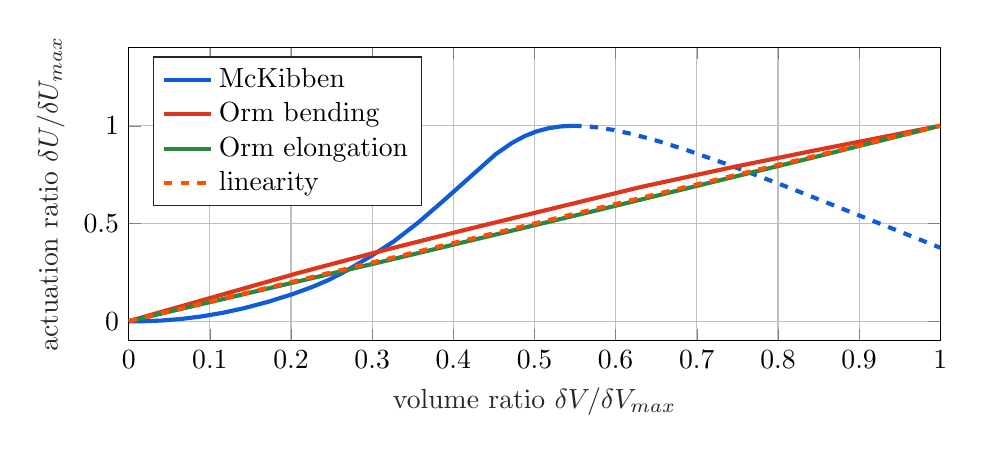
\begin{tikzpicture}

\begin{axis}[%
width=0.85\textwidth,
height=0.307\textwidth,
at={(0\textwidth,0\textwidth)},
scale only axis,
xmin=0,
xmax=1,
xlabel style={font=\color{white!15!black}},
xlabel={volume ratio $\delta V/\delta V_{max}$},
ymin=-0.1,
ymax=1.4,
ylabel style={font=\color{white!15!black}},
ylabel={actuation ratio $\delta U/\delta U_{max}$},
axis background/.style={fill=white},
xmajorgrids,
ymajorgrids,
legend style={at={(0.03,0.97)}, anchor=north west, legend cell align=left, align=left, draw=white!15!black}
]
\addplot [color=mycolor1, line width=1.5pt]
  table[row sep=crcr]{%
0	6.64468480238156e-13\\
0.0201005025125628	8.75243204948584e-05\\
0.0402010050251256	0.00332512405897667\\
0.0653266331658292	0.0117331904478247\\
0.0904522613065327	0.0249046492743175\\
0.115577889447236	0.0427513892029003\\
0.14070351758794	0.0651852988980188\\
0.170854271356784	0.0980369938635274\\
0.201005025125628	0.137215076581811\\
0.226130653266332	0.175068238130177\\
0.246231155778895	0.210907579628632\\
0.266331658291457	0.253741729445041\\
0.301507537688442	0.340391220232792\\
0.326633165829146	0.408312170236871\\
0.35678391959799	0.505004911261358\\
0.386934673366834	0.613214975063938\\
0.452261306532663	0.854807008382492\\
0.472361809045226	0.912631277406958\\
0.487437185929648	0.94626403813337\\
0.50251256281407	0.971128058957608\\
0.517587939698492	0.987706878146325\\
0.532663316582915	0.996954723086223\\
0.547738693467337	0.99999221332643\\
};
\addlegendentry{McKibben}

\addplot [color=mycolor1, dashed, line width=1.5pt, forget plot]
  table[row sep=crcr]{%
0.547738693467337	0.999992213326431\\
0.562814070351759	0.997904288874742\\
0.577889447236181	0.99164328364501\\
0.597989949748744	0.978152194257708\\
0.623115577889447	0.955019458927197\\
0.653266331658292	0.920692312660485\\
0.688442211055276	0.874489150713142\\
0.738693467336683	0.801248259588044\\
0.809045226130653	0.690772107576309\\
0.92964824120603	0.492665242848079\\
1	0.375832322559426\\
};
\addplot [color=mycolor2, line width=1.5pt]
  table[row sep=crcr]{%
0	0\\
0.210526315789474	0.248560359457172\\
0.315789473684211	0.364483047571436\\
0.421052631578947	0.474225435476816\\
0.526315789473684	0.580610711535574\\
0.631578947368421	0.687207531094921\\
0.736842105263158	0.781882023858429\\
0.842105263157895	0.871079842203232\\
1	1\\
};
\addlegendentry{Orm bending}

\addplot [color=mycolor3, line width=1.5pt]
  table[row sep=crcr]{%
0	0\\
0.315789473684211	0.307874524709858\\
0.578947368421053	0.569396702028871\\
0.842105263157895	0.836523467033735\\
1	1\\
};
\addlegendentry{Orm elongation}

\addplot [color=mycolor4, dashed, line width=1.5pt]
  table[row sep=crcr]{%
0	0\\
1	1\\
};
\addlegendentry{linearity}

\end{axis}
\end{tikzpicture}%
  %% This file was created by matlab2tikz.
%
%The latest updates can be retrieved from
%  http://www.mathworks.com/matlabcentral/fileexchange/22022-matlab2tikz-matlab2tikz
%where you can also make suggestions and rate matlab2tikz.
%
\definecolor{mycolor1}{rgb}{0.00000,0.34510,0.65882}%
\definecolor{mycolor2}{rgb}{0.79216,0.11765,0.17255}%
\definecolor{mycolor3}{rgb}{0.80392,0.80392,0.80392}%
%
\begin{tikzpicture}

\begin{axis}[%
width=0.598\textwidth,
height=0.198\textwidth,
at={(0\textwidth,0\textwidth)},
scale only axis,
axis on top,
xmin=0.5,
xmax=1968.5,
tick align=outside,
y dir=reverse,
ymin=0.5,
ymax=650.5,
axis line style={draw=none},
ticks=none
]
\addplot [forget plot] graphics [xmin=0.5, xmax=1968.5, ymin=0.5, ymax=650.5] {fig_bellow-1.png};
\end{axis}

\begin{axis}[%
width=0.297\textwidth,
height=0.192\textwidth,
at={(0.647\textwidth,0.003\textwidth)},
scale only axis,
xmin=0,
xmax=1.5,
xlabel style={font=\color{white!15!black}},
xlabel={pressure (kPa)},
ymin=-10,
ymax=48,
axis background/.style={fill=white},
xmajorgrids,
ymajorgrids,
legend style={at={(0.03,0.97)}, anchor=north west, legend columns=2, legend cell align=left, align=left, draw=white!15!black}
]
\addplot [color=mycolor1, line width=1.5pt]
  table[row sep=crcr]{%
0	0.65625\\
0.020003	0.607624587537979\\
0.0500075000000004	0.52090890773257\\
0.080012	0.424462799914457\\
0.1100165	0.319525122884924\\
0.1500225	0.16696555164601\\
0.1900285	0.000453843840724666\\
0.2300345	-0.179454447130303\\
0.2700405	-0.372153366810661\\
0.320048	-0.630001243232804\\
0.370055499999999	-0.905382412366595\\
0.420063	-1.19674388884769\\
0.480072	-1.56508083669635\\
0.5500825	-2.0165425356607\\
0.6300945	-2.55434051746948\\
0.7501125	-3.38535698180596\\
0.8901335	-4.35081772356119\\
0.960144	-4.81451037470239\\
1.020153	-5.19385040983376\\
1.0701605	-5.4932991768767\\
1.120168	-5.77439258543766\\
1.160174	-5.98401481409548\\
1.20018	-6.1783911802236\\
1.240186	-6.35596306714165\\
1.2701905	-6.47717906047022\\
1.300195	-6.58741633640641\\
1.3301995	-6.68602721835403\\
1.360204	-6.77236958167331\\
1.380207	-6.82280123133512\\
1.40021	-6.86731129683065\\
1.420213	-6.90571514194689\\
1.440216	-6.93782999961751\\
1.460219	-6.96347512113601\\
1.480222	-6.9824719229832\\
1.4999985	-6.99455975856444\\
};
\addlegendentry{volume}

\addplot [color=mycolor2, line width=1.5pt]
  table[row sep=crcr]{%
0	0\\
0.0100015000000013	0.00245869043011382\\
0.0200029999999991	0.0107835674422319\\
0.0300045000000004	0.0255780632427971\\
0.0400060000000018	0.0469985154368366\\
0.0500074999999995	0.0750519434101307\\
0.0600090000000009	0.109696367581613\\
0.0700104999999986	0.150875949865192\\
0.0900135000000013	0.252608954794749\\
0.1100165	0.37979748383194\\
0.1300195	0.531998503555851\\
0.150022499999999	0.708765607964072\\
0.170025500000001	0.909640085412999\\
0.1900285	1.13414697588932\\
0.220033000000001	1.51413512036515\\
0.250037500000001	1.94444209105579\\
0.280041999999998	2.42323219508909\\
0.310046499999999	2.94857465191582\\
0.340050999999999	3.51844359501607\\
0.380057000000001	4.34385328503755\\
0.420062999999999	5.23935282068943\\
0.460069000000001	6.19936000334119\\
0.5100765	7.4811093003182\\
0.560084	8.84236253474872\\
0.620093000000001	10.5627945055091\\
0.690103499999999	12.6602720193967\\
0.80012	16.061668942648\\
0.920137999999998	19.7501049078935\\
0.9901485	21.8053501323974\\
1.040156	23.1979116199186\\
1.0901635	24.5083250390544\\
1.1301695	25.486002185696\\
1.1701755	26.3913519495194\\
1.20018	27.0176133965181\\
1.2301845	27.5945524051951\\
1.260189	28.1184893518037\\
1.2901935	28.5857667374872\\
1.320198	28.9927551662133\\
1.340201	29.228809857066\\
1.360204	29.435415023046\\
1.380207	29.6115236392803\\
1.40021	29.7560980871467\\
1.420213	29.8681109002657\\
1.4302145	29.9115885676228\\
1.440216	29.9465454992476\\
1.4502175	29.9728564423065\\
1.460219	29.9903969139453\\
1.4702205	29.9990432230891\\
1.4902235	30\\
1.4999985	30\\
};
\addlegendentry{$\delta\text{ \!\!L}$}

\end{axis}

\begin{axis}[%
width=1.061\textwidth,
height=0.239\textwidth,
at={(-0.005\textwidth,-0.021\textwidth)},
scale only axis,
xmin=0,
xmax=1,
ymin=0,
ymax=1,
axis line style={draw=none},
ticks=none,
axis x line*=bottom,
axis y line*=left
]
\draw[-{Stealth}, color=mycolor3, line width=1.0pt] (axis cs:0.06,0.03) -- (axis cs:0.55,0.03);
\node[below right, align=left, font=\color{mycolor3}]
at (rel axis cs:0,0.11) {\scriptsize time};
\end{axis}
\end{tikzpicture}%
  \fi
  %\vspace{-6mm}
  \caption{}
\end{figure}
%
\clearpage
}

\newpage
% \begin{figure}[t]
% \centering
% \includegraphics[width=0.98\textwidth]{./3_chapters/0_introduction/img/modern_softrobots.png}
% \caption{\textit{a)} Elepant-inspired trunk [14]. \textit{b)}, Fish-inspired aquatic robot [19]. \textit{c)}, Soft-infalatable human robot arm [13]. \textit{d)}, Concentric-tube hard continuum robot[21]. \textit{e)}, Soft quadruped robot [20]. \textit{f)}. Explosion- driven semi-soft 3D printed robot [22]. }
% \end{figure}

% Perhaps a subtle point in the terminology above, is its mention to biology.
% Although the area of soft robotics has grown exponentially since the early 2010's, the field of soft robotics dates back to the early 60's.

% \begin{figure}
% \centering
% \setlength\figurewidth{0.53\textwidth}
% \setlength\figureheight{0.25\textwidth}
% \input{./3_chapters/0_introduction/img/myfigure.tikz}
% \end{figure}

%\subsection{REF}

The first robotic manipulator arm used in the orbital environment was the Space Shuttle remote manipulator system. It was successfully demonstrated in the STS-2 mission in 1981 and is still operational today.

First soft robot: Victor Scheinman and Larry Leifer developed an air-powered robot arm called Orm, which is the Norwegian word for snake.

% \begin{itemize}
%   \item . F. Shulte, "The Characteristics of the Mckibben Artificial Muscle", The Application of External Power in Prosthetics and Orthetics, pp. 94-115, 1960.
%   \item A. Chen, R. Yin, L. Cao, C. Yuan, H. K. Ding and W. J. Zhang, "Soft robotics: Definition and research issues," 2017 24th International Conference on Mechatronics and Machine Vision in Practice (M2VIP), 2017, pp. 366-370, doi: 10.1109/M2VIP.2017.8267170.
%   \item  W. C. R\"{o}ntgen, “Ueber die durch Electricität bewirkten Form—und Volumenänderungen von dielectrischen Körpern,” Ann Phys Chem, no. 11, pp. 771-786, 1880.
% \end{itemize}


(\textbf{Soft robotics in academia})

\vspace{-4mm}
\section{Challenges in modern soft robotics}
\label{sec:C0:1.2}
%
\begin{figure}[!t]
  \vspace{-2mm}
  \ifx\printFigures\undefined
  \else
  \centering
  \vspace{-2mm}
  % This file was created by matlab2tikz.
%
%The latest updates can be retrieved from
%  http://www.mathworks.com/matlabcentral/fileexchange/22022-matlab2tikz-matlab2tikz
%where you can also make suggestions and rate matlab2tikz.
%
\definecolor{mycolor1}{rgb}{0.06275,0.35686,0.84706}%
\definecolor{mycolor2}{rgb}{0.86667,0.21176,0.10980}%
\definecolor{mycolor3}{rgb}{0.18039,0.52157,0.25098}%
\definecolor{mycolor4}{rgb}{1.00000,0.30980,0.00000}%
%
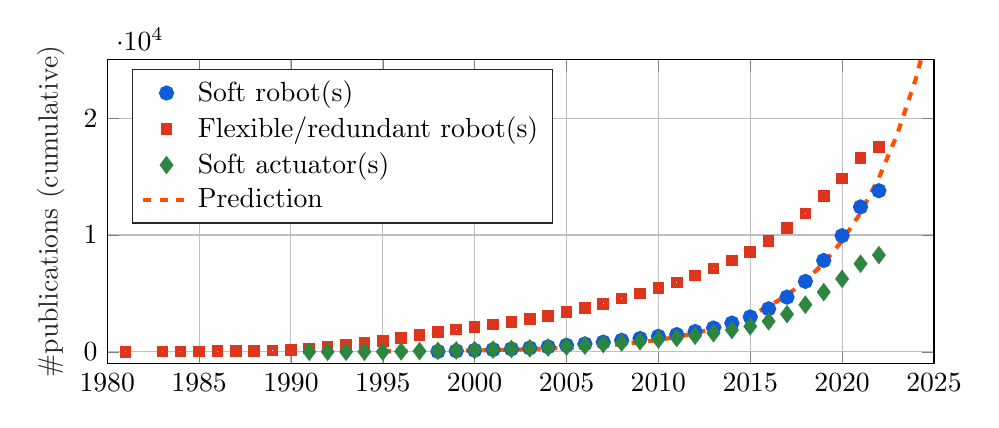
\begin{tikzpicture}

\begin{axis}[%
width=0.866\textwidth,
height=0.318\textwidth,
at={(0\textwidth,0\textwidth)},
scale only axis,
xmin=723181,
xmax=739618,
xtick={723181,725008,726834,728660,730486,732313,734139,735965,737791,739618},
xticklabels={{1980},{1985},{1990},{1995},{2000},{2005},{2010},{2015},{2020},{2025}},
scaled x ticks=false,
ymin=-1000,
ymax=25000,
ylabel style={font=\color{white!15!black}},
ylabel={\#publications (cumulative)},
axis background/.style={fill=white},
xmajorgrids,
ymajorgrids,
legend style={at={(0.03,0.97)}, anchor=north west, legend cell align=left, align=left, draw=white!15!black}
]
\addplot [color=mycolor1, line width=2.0pt, only marks, mark size=1.7pt, mark=*, mark options={solid, mycolor1}]
  table[row sep=crcr]{%
729756	31\\
730121	75\\
730486	125\\
730852	187\\
731217	247\\
731582	327\\
731947	425\\
732313	557\\
732678	675\\
733043	825\\
733408	980\\
733774	1140\\
734139	1318\\
734504	1471\\
734869	1732\\
735235	2039\\
735600	2458\\
735965	2984\\
736330	3680\\
736696	4681\\
737061	6027\\
737426	7816\\
737791	9942\\
738157	12408\\
738522	13791\\
};
\addlegendentry{Soft robot(s)}

\addplot [color=mycolor2, line width=2.0pt, only marks, mark size=1.1pt, mark=square, mark options={solid, mycolor2}]
  table[row sep=crcr]{%
723547	4\\
724277	12\\
724642	19\\
725008	34\\
725373	43\\
725738	58\\
726103	66\\
726469	117\\
726834	168\\
727199	275\\
727564	423\\
727930	582\\
728295	737\\
728660	899\\
729025	1163\\
729391	1423\\
729756	1714\\
730121	1907\\
730486	2109\\
730852	2343\\
731217	2563\\
731582	2818\\
731947	3084\\
732313	3390\\
732678	3741\\
733043	4116\\
733408	4557\\
733774	5007\\
734139	5482\\
734504	5936\\
734869	6529\\
735235	7133\\
735600	7826\\
735965	8563\\
736330	9482\\
736696	10586\\
737061	11827\\
737426	13342\\
737791	14847\\
738157	16584\\
738522	17555\\
};
\addlegendentry{Flexible/redundant robot(s)}

\addplot [color=mycolor3, line width=2.0pt, only marks, mark size=1.7pt, mark=diamond, mark options={solid, mycolor3}]
  table[row sep=crcr]{%
727199	1\\
727564	2\\
727930	4\\
728295	9\\
728660	12\\
729025	28\\
729391	55\\
729756	81\\
730121	118\\
730486	153\\
730852	190\\
731217	240\\
731582	294\\
731947	365\\
732313	439\\
732678	533\\
733043	662\\
733408	783\\
733774	894\\
734139	1050\\
734504	1179\\
734869	1375\\
735235	1584\\
735600	1864\\
735965	2175\\
736330	2612\\
736696	3218\\
737061	4031\\
737426	5109\\
737791	6243\\
738157	7542\\
738522	8281\\
};
\addlegendentry{Soft actuator(s)}

\addplot [color=mycolor4, dashed, line width=1.5pt]
  table[row sep=crcr]{%
728660	44.6634216554798\\
728660	44.6634216554798\\
728660	44.6634216554798\\
728660	44.6634216554798\\
728660	44.6634216554798\\
728660	44.6634216554798\\
728660	44.6634216554798\\
728660	44.6634216554798\\
728660	44.6634216554798\\
728660	44.6634216554798\\
728660	44.6634216554798\\
728660	44.6634216554798\\
728660	44.6634216554798\\
728660	44.6634216554798\\
728660	44.6634216554798\\
728660	44.6634216554798\\
728660	44.6634216554798\\
729025	53.3890888278004\\
729025	53.3890888278004\\
729025	53.3890888278004\\
729025	53.3890888278004\\
729025	53.3890888278004\\
729025	53.3890888278004\\
729025	53.3890888278004\\
729025	53.3890888278004\\
729025	53.3890888278004\\
729025	53.3890888278004\\
729025	53.3890888278004\\
729025	53.3890888278004\\
729025	53.3890888278004\\
729025	53.3890888278004\\
729025	53.3890888278004\\
729025	53.3890888278004\\
729025	53.3890888278004\\
729025	53.3890888278004\\
729025	53.3890888278004\\
729025	53.3890888278004\\
729025	53.3890888278004\\
729025	53.3890888278004\\
729025	53.3890888278004\\
729025	53.3890888278004\\
729025	53.3890888278004\\
729025	53.3890888278004\\
729025	53.3890888278004\\
729025	53.3890888278004\\
729025	53.3890888278004\\
729025	53.3890888278004\\
729025	53.3890888278004\\
729025	53.3890888278004\\
729025	53.3890888278004\\
729391	64.3112289380452\\
729391	64.3112289380452\\
729391	64.3112289380452\\
729391	64.3112289380452\\
729391	64.3112289380452\\
729391	64.3112289380452\\
729391	64.3112289380452\\
729391	64.3112289380452\\
729391	64.3112289380452\\
729391	64.3112289380452\\
729391	64.3112289380452\\
729391	64.3112289380452\\
729391	64.3112289380452\\
729391	64.3112289380452\\
729391	64.3112289380452\\
729391	64.3112289380452\\
729391	64.3112289380452\\
729391	64.3112289380452\\
729391	64.3112289380452\\
729391	64.3112289380452\\
729391	64.3112289380452\\
729391	64.3112289380452\\
729391	64.3112289380452\\
729391	64.3112289380452\\
729391	64.3112289380452\\
729391	64.3112289380452\\
729391	64.3112289380452\\
729391	64.3112289380452\\
729391	64.3112289380452\\
729391	64.3112289380452\\
729391	64.3112289380452\\
729391	64.3112289380452\\
729391	64.3112289380452\\
729391	64.3112289380452\\
729756	77.9827502362947\\
729756	77.9827502362947\\
729756	77.9827502362947\\
729756	77.9827502362947\\
729756	77.9827502362947\\
729756	77.9827502362947\\
729756	77.9827502362947\\
729756	77.9827502362947\\
729756	77.9827502362947\\
729756	77.9827502362947\\
729756	77.9827502362947\\
729756	77.9827502362947\\
729756	77.9827502362947\\
729756	77.9827502362947\\
729756	77.9827502362947\\
729756	77.9827502362947\\
729756	77.9827502362947\\
729756	77.9827502362947\\
729756	77.9827502362947\\
729756	77.9827502362947\\
729756	77.9827502362947\\
729756	77.9827502362947\\
729756	77.9827502362947\\
729756	77.9827502362947\\
729756	77.9827502362947\\
729756	77.9827502362947\\
729756	77.9827502362947\\
729756	77.9827502362947\\
729756	77.9827502362947\\
729756	77.9827502362947\\
729756	77.9827502362947\\
729756	77.9827502362947\\
729756	77.9827502362947\\
730121	95.095742078724\\
730121	95.095742078724\\
730121	95.095742078724\\
730121	95.095742078724\\
730121	95.095742078724\\
730121	95.095742078724\\
730121	95.095742078724\\
730121	95.095742078724\\
730121	95.095742078724\\
730121	95.095742078724\\
730121	95.095742078724\\
730121	95.095742078724\\
730121	95.095742078724\\
730121	95.095742078724\\
730121	95.095742078724\\
730121	95.095742078724\\
730121	95.095742078724\\
730121	95.095742078724\\
730121	95.095742078724\\
730121	95.095742078724\\
730121	95.095742078724\\
730121	95.095742078724\\
730121	95.095742078724\\
730121	95.095742078724\\
730121	95.095742078724\\
730121	95.095742078724\\
730121	95.095742078724\\
730121	95.095742078724\\
730121	95.095742078724\\
730121	95.095742078724\\
730121	95.095742078724\\
730121	95.095742078724\\
730121	95.095742078724\\
730486	116.516510361223\\
730486	116.516510361223\\
730486	116.516510361223\\
730486	116.516510361223\\
730486	116.516510361223\\
730486	116.516510361223\\
730486	116.516510361223\\
730486	116.516510361223\\
730486	116.516510361223\\
730486	116.516510361223\\
730486	116.516510361223\\
730486	116.516510361223\\
730486	116.516510361223\\
730486	116.516510361223\\
730486	116.516510361223\\
730486	116.516510361223\\
730486	116.516510361223\\
730486	116.516510361223\\
730486	116.516510361223\\
730486	116.516510361223\\
730486	116.516510361223\\
730486	116.516510361223\\
730486	116.516510361223\\
730486	116.516510361223\\
730486	116.516510361223\\
730486	116.516510361223\\
730486	116.516510361223\\
730486	116.516510361223\\
730486	116.516510361223\\
730486	116.516510361223\\
730486	116.516510361223\\
730486	116.516510361223\\
730486	116.516510361223\\
730486	116.516510361223\\
730852	143.329432265087\\
730852	143.329432265087\\
730852	143.329432265087\\
730852	143.329432265087\\
730852	143.329432265087\\
730852	143.329432265087\\
730852	143.329432265087\\
730852	143.329432265087\\
730852	143.329432265087\\
730852	143.329432265087\\
730852	143.329432265087\\
730852	143.329432265087\\
730852	143.329432265087\\
730852	143.329432265087\\
730852	143.329432265087\\
730852	143.329432265087\\
730852	143.329432265087\\
730852	143.329432265087\\
730852	143.329432265087\\
730852	143.329432265087\\
730852	143.329432265087\\
730852	143.329432265087\\
730852	143.329432265087\\
730852	143.329432265087\\
730852	143.329432265087\\
730852	143.329432265087\\
730852	143.329432265087\\
730852	143.329432265087\\
730852	143.329432265087\\
730852	143.329432265087\\
730852	143.329432265087\\
730852	143.329432265087\\
730852	143.329432265087\\
731217	176.891850360523\\
731217	176.891850360523\\
731217	176.891850360523\\
731217	176.891850360523\\
731217	176.891850360523\\
731217	176.891850360523\\
731217	176.891850360523\\
731217	176.891850360523\\
731217	176.891850360523\\
731217	176.891850360523\\
731217	176.891850360523\\
731217	176.891850360523\\
731217	176.891850360523\\
731217	176.891850360523\\
731217	176.891850360523\\
731217	176.891850360523\\
731217	176.891850360523\\
731217	176.891850360523\\
731217	176.891850360523\\
731217	176.891850360523\\
731217	176.891850360523\\
731217	176.891850360523\\
731217	176.891850360523\\
731217	176.891850360523\\
731217	176.891850360523\\
731217	176.891850360523\\
731217	176.891850360523\\
731217	176.891850360523\\
731217	176.891850360523\\
731217	176.891850360523\\
731217	176.891850360523\\
731217	176.891850360523\\
731217	176.891850360523\\
731582	218.902784955852\\
731582	218.902784955852\\
731582	218.902784955852\\
731582	218.902784955852\\
731582	218.902784955852\\
731582	218.902784955852\\
731582	218.902784955852\\
731582	218.902784955852\\
731582	218.902784955852\\
731582	218.902784955852\\
731582	218.902784955852\\
731582	218.902784955852\\
731582	218.902784955852\\
731582	218.902784955852\\
731582	218.902784955852\\
731582	218.902784955852\\
731582	218.902784955852\\
731582	218.902784955852\\
731582	218.902784955852\\
731582	218.902784955852\\
731582	218.902784955852\\
731582	218.902784955852\\
731582	218.902784955852\\
731582	218.902784955852\\
731582	218.902784955852\\
731582	218.902784955852\\
731582	218.902784955852\\
731582	218.902784955852\\
731582	218.902784955852\\
731582	218.902784955852\\
731582	218.902784955852\\
731582	218.902784955852\\
731582	218.902784955852\\
731582	218.902784955852\\
731947	271.48894309721\\
731947	271.48894309721\\
731947	271.48894309721\\
731947	271.48894309721\\
731947	271.48894309721\\
731947	271.48894309721\\
731947	271.48894309721\\
731947	271.48894309721\\
731947	271.48894309721\\
731947	271.48894309721\\
731947	271.48894309721\\
731947	271.48894309721\\
731947	271.48894309721\\
731947	271.48894309721\\
731947	271.48894309721\\
731947	271.48894309721\\
731947	271.48894309721\\
731947	271.48894309721\\
731947	271.48894309721\\
731947	271.48894309721\\
731947	271.48894309721\\
731947	271.48894309721\\
731947	271.48894309721\\
731947	271.48894309721\\
731947	271.48894309721\\
731947	271.48894309721\\
731947	271.48894309721\\
731947	271.48894309721\\
731947	271.48894309721\\
731947	271.48894309721\\
731947	271.48894309721\\
731947	271.48894309721\\
731947	271.48894309721\\
732313	337.312378226773\\
732313	337.312378226773\\
732313	337.312378226773\\
732313	337.312378226773\\
732313	337.312378226773\\
732313	337.312378226773\\
732313	337.312378226773\\
732313	337.312378226773\\
732313	337.312378226773\\
732313	337.312378226773\\
732313	337.312378226773\\
732313	337.312378226773\\
732313	337.312378226773\\
732313	337.312378226773\\
732313	337.312378226773\\
732313	337.312378226773\\
732313	337.312378226773\\
732313	337.312378226773\\
732313	337.312378226773\\
732313	337.312378226773\\
732313	337.312378226773\\
732313	337.312378226773\\
732313	337.312378226773\\
732313	337.312378226773\\
732313	337.312378226773\\
732313	337.312378226773\\
732313	337.312378226773\\
732313	337.312378226773\\
732313	337.312378226773\\
732313	337.312378226773\\
732313	337.312378226773\\
732313	337.312378226773\\
732313	337.312378226773\\
732678	419.705250522346\\
732678	419.705250522346\\
732678	419.705250522346\\
732678	419.705250522346\\
732678	419.705250522346\\
732678	419.705250522346\\
732678	419.705250522346\\
732678	419.705250522346\\
732678	419.705250522346\\
732678	419.705250522346\\
732678	419.705250522346\\
732678	419.705250522346\\
732678	419.705250522346\\
732678	419.705250522346\\
732678	419.705250522346\\
732678	419.705250522346\\
732678	419.705250522346\\
732678	419.705250522346\\
732678	419.705250522346\\
732678	419.705250522346\\
732678	419.705250522346\\
732678	419.705250522346\\
732678	419.705250522346\\
732678	419.705250522346\\
732678	419.705250522346\\
732678	419.705250522346\\
732678	419.705250522346\\
732678	419.705250522346\\
732678	419.705250522346\\
732678	419.705250522346\\
732678	419.705250522346\\
732678	419.705250522346\\
732678	419.705250522346\\
733043	522.838509850919\\
733043	522.838509850919\\
733043	522.838509850919\\
733043	522.838509850919\\
733043	522.838509850919\\
733043	522.838509850919\\
733043	522.838509850919\\
733043	522.838509850919\\
733043	522.838509850919\\
733043	522.838509850919\\
733043	522.838509850919\\
733043	522.838509850919\\
733043	522.838509850919\\
733043	522.838509850919\\
733043	522.838509850919\\
733043	522.838509850919\\
733043	522.838509850919\\
733043	522.838509850919\\
733043	522.838509850919\\
733043	522.838509850919\\
733043	522.838509850919\\
733043	522.838509850919\\
733043	522.838509850919\\
733043	522.838509850919\\
733043	522.838509850919\\
733043	522.838509850919\\
733043	522.838509850919\\
733043	522.838509850919\\
733043	522.838509850919\\
733043	522.838509850919\\
733043	522.838509850919\\
733043	522.838509850919\\
733043	522.838509850919\\
733043	522.838509850919\\
733408	651.933040523155\\
733408	651.933040523155\\
733408	651.933040523155\\
733408	651.933040523155\\
733408	651.933040523155\\
733408	651.933040523155\\
733408	651.933040523155\\
733408	651.933040523155\\
733408	651.933040523155\\
733408	651.933040523155\\
733408	651.933040523155\\
733408	651.933040523155\\
733408	651.933040523155\\
733408	651.933040523155\\
733408	651.933040523155\\
733408	651.933040523155\\
733408	651.933040523155\\
733408	651.933040523155\\
733408	651.933040523155\\
733408	651.933040523155\\
733408	651.933040523155\\
733408	651.933040523155\\
733408	651.933040523155\\
733408	651.933040523155\\
733408	651.933040523155\\
733408	651.933040523155\\
733408	651.933040523155\\
733408	651.933040523155\\
733408	651.933040523155\\
733408	651.933040523155\\
733408	651.933040523155\\
733408	651.933040523155\\
733408	651.933040523155\\
733774	813.523956566939\\
733774	813.523956566939\\
733774	813.523956566939\\
733774	813.523956566939\\
733774	813.523956566939\\
733774	813.523956566939\\
733774	813.523956566939\\
733774	813.523956566939\\
733774	813.523956566939\\
733774	813.523956566939\\
733774	813.523956566939\\
733774	813.523956566939\\
733774	813.523956566939\\
733774	813.523956566939\\
733774	813.523956566939\\
733774	813.523956566939\\
733774	813.523956566939\\
733774	813.523956566939\\
733774	813.523956566939\\
733774	813.523956566939\\
733774	813.523956566939\\
733774	813.523956566939\\
733774	813.523956566939\\
733774	813.523956566939\\
733774	813.523956566939\\
733774	813.523956566939\\
733774	813.523956566939\\
733774	813.523956566939\\
733774	813.523956566939\\
733774	813.523956566939\\
733774	813.523956566939\\
733774	813.523956566939\\
733774	813.523956566939\\
734139	1015.79142686097\\
734139	1015.79142686097\\
734139	1015.79142686097\\
734139	1015.79142686097\\
734139	1015.79142686097\\
734139	1015.79142686097\\
734139	1015.79142686097\\
734139	1015.79142686097\\
734139	1015.79142686097\\
734139	1015.79142686097\\
734139	1015.79142686097\\
734139	1015.79142686097\\
734139	1015.79142686097\\
734139	1015.79142686097\\
734139	1015.79142686097\\
734139	1015.79142686097\\
734139	1015.79142686097\\
734139	1015.79142686097\\
734139	1015.79142686097\\
734139	1015.79142686097\\
734139	1015.79142686097\\
734139	1015.79142686097\\
734139	1015.79142686097\\
734139	1015.79142686097\\
734139	1015.79142686097\\
734139	1015.79142686097\\
734139	1015.79142686097\\
734139	1015.79142686097\\
734139	1015.79142686097\\
734139	1015.79142686097\\
734139	1015.79142686097\\
734139	1015.79142686097\\
734139	1015.79142686097\\
734139	1015.79142686097\\
734504	1268.97477739086\\
734504	1268.97477739086\\
734504	1268.97477739086\\
734504	1268.97477739086\\
734504	1268.97477739086\\
734504	1268.97477739086\\
734504	1268.97477739086\\
734504	1268.97477739086\\
734504	1268.97477739086\\
734504	1268.97477739086\\
734504	1268.97477739086\\
734504	1268.97477739086\\
734504	1268.97477739086\\
734504	1268.97477739086\\
734504	1268.97477739086\\
734504	1268.97477739086\\
734504	1268.97477739086\\
734504	1268.97477739086\\
734504	1268.97477739086\\
734504	1268.97477739086\\
734504	1268.97477739086\\
734504	1268.97477739086\\
734504	1268.97477739086\\
734504	1268.97477739086\\
734504	1268.97477739086\\
734504	1268.97477739086\\
734504	1268.97477739086\\
734504	1268.97477739086\\
734504	1268.97477739086\\
734504	1268.97477739086\\
734504	1268.97477739086\\
734504	1268.97477739086\\
734504	1268.97477739086\\
734869	1585.89083360259\\
734869	1585.89083360259\\
734869	1585.89083360259\\
734869	1585.89083360259\\
734869	1585.89083360259\\
734869	1585.89083360259\\
734869	1585.89083360259\\
734869	1585.89083360259\\
734869	1585.89083360259\\
734869	1585.89083360259\\
734869	1585.89083360259\\
734869	1585.89083360259\\
734869	1585.89083360259\\
734869	1585.89083360259\\
734869	1585.89083360259\\
734869	1585.89083360259\\
734869	1585.89083360259\\
734869	1585.89083360259\\
734869	1585.89083360259\\
734869	1585.89083360259\\
734869	1585.89083360259\\
734869	1585.89083360259\\
734869	1585.89083360259\\
734869	1585.89083360259\\
734869	1585.89083360259\\
734869	1585.89083360259\\
734869	1585.89083360259\\
734869	1585.89083360259\\
734869	1585.89083360259\\
734869	1585.89083360259\\
734869	1585.89083360259\\
734869	1585.89083360259\\
734869	1585.89083360259\\
735235	1982.58274274519\\
735235	1982.58274274519\\
735235	1982.58274274519\\
735235	1982.58274274519\\
735235	1982.58274274519\\
735235	1982.58274274519\\
735235	1982.58274274519\\
735235	1982.58274274519\\
735235	1982.58274274519\\
735235	1982.58274274519\\
735235	1982.58274274519\\
735235	1982.58274274519\\
735235	1982.58274274519\\
735235	1982.58274274519\\
735235	1982.58274274519\\
735235	1982.58274274519\\
735235	1982.58274274519\\
735235	1982.58274274519\\
735235	1982.58274274519\\
735235	1982.58274274519\\
735235	1982.58274274519\\
735235	1982.58274274519\\
735235	1982.58274274519\\
735235	1982.58274274519\\
735235	1982.58274274519\\
735235	1982.58274274519\\
735235	1982.58274274519\\
735235	1982.58274274519\\
735235	1982.58274274519\\
735235	1982.58274274519\\
735235	1982.58274274519\\
735235	1982.58274274519\\
735235	1982.58274274519\\
735235	1982.58274274519\\
735600	2479.13212134172\\
735600	2479.13212134172\\
735600	2479.13212134172\\
735600	2479.13212134172\\
735600	2479.13212134172\\
735600	2479.13212134172\\
735600	2479.13212134172\\
735600	2479.13212134172\\
735600	2479.13212134172\\
735600	2479.13212134172\\
735600	2479.13212134172\\
735600	2479.13212134172\\
735600	2479.13212134172\\
735600	2479.13212134172\\
735600	2479.13212134172\\
735600	2479.13212134172\\
735600	2479.13212134172\\
735600	2479.13212134172\\
735600	2479.13212134172\\
735600	2479.13212134172\\
735600	2479.13212134172\\
735600	2479.13212134172\\
735600	2479.13212134172\\
735600	2479.13212134172\\
735600	2479.13212134172\\
735600	2479.13212134172\\
735600	2479.13212134172\\
735600	2479.13212134172\\
735600	2479.13212134172\\
735600	2479.13212134172\\
735600	2479.13212134172\\
735600	2479.13212134172\\
735600	2479.13212134172\\
735965	3100.67564088946\\
735965	3100.67564088946\\
735965	3100.67564088946\\
735965	3100.67564088946\\
735965	3100.67564088946\\
735965	3100.67564088946\\
735965	3100.67564088946\\
735965	3100.67564088946\\
735965	3100.67564088946\\
735965	3100.67564088946\\
735965	3100.67564088946\\
735965	3100.67564088946\\
735965	3100.67564088946\\
735965	3100.67564088946\\
735965	3100.67564088946\\
735965	3100.67564088946\\
735965	3100.67564088946\\
735965	3100.67564088946\\
735965	3100.67564088946\\
735965	3100.67564088946\\
735965	3100.67564088946\\
735965	3100.67564088946\\
735965	3100.67564088946\\
735965	3100.67564088946\\
735965	3100.67564088946\\
735965	3100.67564088946\\
735965	3100.67564088946\\
735965	3100.67564088946\\
735965	3100.67564088946\\
735965	3100.67564088946\\
735965	3100.67564088946\\
735965	3100.67564088946\\
735965	3100.67564088946\\
736330	3878.67751410433\\
736330	3878.67751410433\\
736330	3878.67751410433\\
736330	3878.67751410433\\
736330	3878.67751410433\\
736330	3878.67751410433\\
736330	3878.67751410433\\
736330	3878.67751410433\\
736330	3878.67751410433\\
736330	3878.67751410433\\
736330	3878.67751410433\\
736330	3878.67751410433\\
736330	3878.67751410433\\
736330	3878.67751410433\\
736330	3878.67751410433\\
736330	3878.67751410433\\
736330	3878.67751410433\\
736330	3878.67751410433\\
736330	3878.67751410433\\
736330	3878.67751410433\\
736330	3878.67751410433\\
736330	3878.67751410433\\
736330	3878.67751410433\\
736330	3878.67751410433\\
736330	3878.67751410433\\
736330	3878.67751410433\\
736330	3878.67751410433\\
736330	3878.67751410433\\
736330	3878.67751410433\\
736330	3878.67751410433\\
736330	3878.67751410433\\
736330	3878.67751410433\\
736330	3878.67751410433\\
736696	4852.52229840244\\
736696	4852.52229840244\\
736696	4852.52229840244\\
736696	4852.52229840244\\
736696	4852.52229840244\\
736696	4852.52229840244\\
736696	4852.52229840244\\
736696	4852.52229840244\\
736696	4852.52229840244\\
736696	4852.52229840244\\
736696	4852.52229840244\\
736696	4852.52229840244\\
736696	4852.52229840244\\
736696	4852.52229840244\\
736696	4852.52229840244\\
736696	4852.52229840244\\
736696	4852.52229840244\\
736696	4852.52229840244\\
736696	4852.52229840244\\
736696	4852.52229840244\\
736696	4852.52229840244\\
736696	4852.52229840244\\
736696	4852.52229840244\\
736696	4852.52229840244\\
736696	4852.52229840244\\
736696	4852.52229840244\\
736696	4852.52229840244\\
736696	4852.52229840244\\
736696	4852.52229840244\\
736696	4852.52229840244\\
736696	4852.52229840244\\
736696	4852.52229840244\\
736696	4852.52229840244\\
736696	4852.52229840244\\
737061	6071.50864863545\\
737061	6071.50864863545\\
737061	6071.50864863545\\
737061	6071.50864863545\\
737061	6071.50864863545\\
737061	6071.50864863545\\
737061	6071.50864863545\\
737061	6071.50864863545\\
737061	6071.50864863545\\
737061	6071.50864863545\\
737061	6071.50864863545\\
737061	6071.50864863545\\
737061	6071.50864863545\\
737061	6071.50864863545\\
737061	6071.50864863545\\
737061	6071.50864863545\\
737061	6071.50864863545\\
737061	6071.50864863545\\
737061	6071.50864863545\\
737061	6071.50864863545\\
737061	6071.50864863545\\
737061	6071.50864863545\\
737061	6071.50864863545\\
737061	6071.50864863545\\
737061	6071.50864863545\\
737061	6071.50864863545\\
737061	6071.50864863545\\
737061	6071.50864863545\\
737061	6071.50864863545\\
737061	6071.50864863545\\
737061	6071.50864863545\\
737061	6071.50864863545\\
737061	6071.50864863545\\
737426	7597.34494823154\\
737426	7597.34494823154\\
737426	7597.34494823154\\
737426	7597.34494823154\\
737426	7597.34494823154\\
737426	7597.34494823154\\
737426	7597.34494823154\\
737426	7597.34494823154\\
737426	7597.34494823154\\
737426	7597.34494823154\\
737426	7597.34494823154\\
737426	7597.34494823154\\
737426	7597.34494823154\\
737426	7597.34494823154\\
737426	7597.34494823154\\
737426	7597.34494823154\\
737426	7597.34494823154\\
737426	7597.34494823154\\
737426	7597.34494823154\\
737426	7597.34494823154\\
737426	7597.34494823154\\
737426	7597.34494823154\\
737426	7597.34494823154\\
737426	7597.34494823154\\
737426	7597.34494823154\\
737426	7597.34494823154\\
737426	7597.34494823154\\
737426	7597.34494823154\\
737426	7597.34494823154\\
737426	7597.34494823154\\
737426	7597.34494823154\\
737426	7597.34494823154\\
737426	7597.34494823154\\
737791	9507.27315433496\\
737791	9507.27315433496\\
737791	9507.27315433496\\
737791	9507.27315433496\\
737791	9507.27315433496\\
737791	9507.27315433496\\
737791	9507.27315433496\\
737791	9507.27315433496\\
737791	9507.27315433496\\
737791	9507.27315433496\\
737791	9507.27315433496\\
737791	9507.27315433496\\
737791	9507.27315433496\\
737791	9507.27315433496\\
737791	9507.27315433496\\
737791	9507.27315433496\\
737791	9507.27315433496\\
737791	9507.27315433496\\
737791	9507.27315433496\\
737791	9507.27315433496\\
737791	9507.27315433496\\
737791	9507.27315433496\\
737791	9507.27315433496\\
737791	9507.27315433496\\
737791	9507.27315433496\\
737791	9507.27315433496\\
737791	9507.27315433496\\
737791	9507.27315433496\\
737791	9507.27315433496\\
737791	9507.27315433496\\
737791	9507.27315433496\\
737791	9507.27315433496\\
737791	9507.27315433496\\
737791	9507.27315433496\\
738157	11897.9789944274\\
738157	11897.9789944274\\
738157	11897.9789944274\\
738157	11897.9789944274\\
738157	11897.9789944274\\
738157	11897.9789944274\\
738157	11897.9789944274\\
738157	11897.9789944274\\
738157	11897.9789944274\\
738157	11897.9789944274\\
738157	11897.9789944274\\
738157	11897.9789944274\\
738157	11897.9789944274\\
738157	11897.9789944274\\
738157	11897.9789944274\\
738157	11897.9789944274\\
738157	11897.9789944274\\
738157	11897.9789944274\\
738157	11897.9789944274\\
738157	11897.9789944274\\
738157	11897.9789944274\\
738157	11897.9789944274\\
738157	11897.9789944274\\
738157	11897.9789944274\\
738157	11897.9789944274\\
738157	11897.9789944274\\
738157	11897.9789944274\\
738157	11897.9789944274\\
738157	11897.9789944274\\
738157	11897.9789944274\\
738157	11897.9789944274\\
738157	11897.9789944274\\
738157	11897.9789944274\\
738522	14890.4864591518\\
738522	14890.4864591518\\
738522	14890.4864591518\\
738522	14890.4864591518\\
738522	14890.4864591518\\
738522	14890.4864591518\\
738522	14890.4864591518\\
738522	14890.4864591518\\
738522	14890.4864591518\\
738522	14890.4864591518\\
738522	14890.4864591518\\
738522	14890.4864591518\\
738522	14890.4864591518\\
738522	14890.4864591518\\
738522	14890.4864591518\\
738522	14890.4864591518\\
738522	14890.4864591518\\
738522	14890.4864591518\\
738522	14890.4864591518\\
738522	14890.4864591518\\
738522	14890.4864591518\\
738522	14890.4864591518\\
738522	14890.4864591518\\
738522	14890.4864591518\\
738522	14890.4864591518\\
738522	14890.4864591518\\
738522	14890.4864591518\\
738522	14890.4864591518\\
738522	14890.4864591518\\
738522	14890.4864591518\\
738522	14890.4864591518\\
738522	14890.4864591518\\
738522	14890.4864591518\\
738887	18636.2843637928\\
738887	18636.2843637928\\
738887	18636.2843637928\\
738887	18636.2843637928\\
738887	18636.2843637928\\
738887	18636.2843637928\\
738887	18636.2843637928\\
738887	18636.2843637928\\
738887	18636.2843637928\\
738887	18636.2843637928\\
738887	18636.2843637928\\
738887	18636.2843637928\\
738887	18636.2843637928\\
738887	18636.2843637928\\
738887	18636.2843637928\\
738887	18636.2843637928\\
738887	18636.2843637928\\
738887	18636.2843637928\\
738887	18636.2843637928\\
738887	18636.2843637928\\
738887	18636.2843637928\\
738887	18636.2843637928\\
738887	18636.2843637928\\
738887	18636.2843637928\\
738887	18636.2843637928\\
738887	18636.2843637928\\
738887	18636.2843637928\\
738887	18636.2843637928\\
738887	18636.2843637928\\
738887	18636.2843637928\\
738887	18636.2843637928\\
738887	18636.2843637928\\
738887	18636.2843637928\\
738887	18636.2843637928\\
739252	23324.9951215135\\
739252	23324.9951215135\\
739252	23324.9951215135\\
739252	23324.9951215135\\
739252	23324.9951215135\\
739252	23324.9951215135\\
739252	23324.9951215135\\
739252	23324.9951215135\\
739252	23324.9951215135\\
739252	23324.9951215135\\
739252	23324.9951215135\\
739252	23324.9951215135\\
739252	23324.9951215135\\
739252	23324.9951215135\\
739252	23324.9951215135\\
739252	23324.9951215135\\
739252	23324.9951215135\\
739252	23324.9951215135\\
739252	23324.9951215135\\
739252	23324.9951215135\\
739252	23324.9951215135\\
739252	23324.9951215135\\
739252	23324.9951215135\\
739252	23324.9951215135\\
739252	23324.9951215135\\
739252	23324.9951215135\\
739252	23324.9951215135\\
739252	23324.9951215135\\
739252	23324.9951215135\\
739252	23324.9951215135\\
739252	23324.9951215135\\
739252	23324.9951215135\\
739252	23324.9951215135\\
739618	29193.9739423751\\
739618	29193.9739423751\\
739618	29193.9739423751\\
739618	29193.9739423751\\
739618	29193.9739423751\\
739618	29193.9739423751\\
739618	29193.9739423751\\
739618	29193.9739423751\\
739618	29193.9739423751\\
739618	29193.9739423751\\
739618	29193.9739423751\\
739618	29193.9739423751\\
739618	29193.9739423751\\
739618	29193.9739423751\\
739618	29193.9739423751\\
739618	29193.9739423751\\
739618	29193.9739423751\\
};
\addlegendentry{Prediction}

\end{axis}
\end{tikzpicture}%
  \fi
  \vspace{-1mm}
  \caption{Cumulative number of (scientific) publications on the topic of \emph{soft robots} or related topics. Data acquired from the Web of Sciences data repository.}
  \vspace{-3mm}
  \label{fig:C0:publicationhistory}
\end{figure}
%
The exact date of the academic boom of soft robotics is unclear, but it is believed to be the mid 2000's. To motivate the argument, we have provided a graph of scientific publications on the topic \textit{soft robot(s)} from 1980 till 2022 (see Figure \ref{fig:C0:publicationhistory}). It shows the cumulative number of publications related to the term soft robot in the titles, keywords, and abstracts. The publication data from Figure \ref{fig:C0:publicationhistory} is obtained using the Web of Sciences data repository. Let it be clear that the term \textit{soft robot} was introduced decades after hyper-redundant robots, thus some older academic work might be lost simply due to different terminology. Hence, we also provided related topics such as '\textit{flexible}' and '\textit{redundant robot(s)}'. In the following section, we will discuss modern trends and challenges in the field of soft robotics, that continue the research paths of highly-flexible robots in early 90's.

\begin{rmk}In retrospect to the previous section, soft robotics is an extensive and diverse academic field since early 90's and it has been growing ever since. Given its vastness, we will limit our scope here. Within the upcoming introductory material, we will primarily focus on topics related to: $(i)$ categories in soft robotics, \eg, soft grippers and manipulators, $(ii)$ design and fabrication of fluidic soft actuators, and $(iii)$ modelling and control for the soft manipulator subclass.
\end{rmk}

\vspace{-4mm}
\subsection{Labelling of soft robotic systems}
In the past two decades, soft robotics has undergone an evolutionary-like transformation alike biological systems. In this section, we humbly attempt to  categorize some soft robotic systems. 

\textbf{Soft grippers}. Although the origin of soft robots might stem from manipulators, modern soft robotics is perhaps most known for its diversity in soft grippers. Many systems explore redundancy and adaptability in grasping -- and its subsequent manipulation of objects of various sizes, densities, compliance, and fragility. This subfield is a direct response to the hurdles in rigid robotics, where sensory force feedback and strict control laws are necessary for simultaneous safe and firm grasping. Soft grippers, on the other hand, have the natural advantage of adapting to shape and compliance of objects without the need for advanced controllers. Recalling the work of Suzumori et al. \cite{Suzumori1991,Suzumori1992} and earlier the work of Teleshev \cite{Teleshev1981}, many soft grippers explore pneumatics or hydraulics for joint motion. These inherently under-actuated soft grippers, often composed of silicone with embedded pneumatic, have shown impressive adaptability and dexterity in recent years \cite{Ilievski2011Feb,Deimel2015Aug}. Galloway et al. (2016, \cite{Galloway2016}) developed an underwater soft gripper to delicately manipulate and sample fragile species on the deep reef (see Figure \ref{fig:C0:typesofrobots}a). Their deep-reef grippers are inspired by the PneuNet actuators from Mosadegh et al. (2014, \cite{Mosadegh2014}). Li et al. (2017, \cite{Li2017Dec}) developed enveloping soft grippers by combining collapsible origami structures enveloped in flexible skin. Hong et al. (2022, \cite{Hong2022Jan}) explored kirigami soft grippers, delicate enough to handle the yolk of an egg. Others explore electro-adhesive soft grippers, like Shintake et al. (2016, \cite{Shintake2016Jan}) and Dadkhah et al. (2016, \cite{Dadkhah2016}), that can manipulate an unprecedented range of object types. By far, these systems have matured the most, even employing the technology in many industrial and commercial applications \cite{Labs2021Jul,Ansari2022Sep}.
%
\begin{figure}[!t]
  \vspace{-2mm}
  \ifx\printFigures\undefined
  \else
  \centering
  \hspace{2mm}
  %\input{/home/brandon/Documents/phd/thesis/3_chapters/0_introduction/img/fig_robot_types.tex}
  \vspace{-7mm}
  \fi
  %
  \caption{Various categories in soft robotic systems. (a) Soft grippers by Galloway et al. (2016, \cite{Galloway2016}). (b) Commercial soft continuum manipulator by Festo Inc. \cite{Gravagne2001Oct} (c) Soft continuum Proprioceptive Arm (SoPrA) by Toshimitsu et al. (2021, \cite{Toshimitsu2021Sep,Wand2022Apr}). (d) Soft robotic fish by Katzschmann et al. (2018, \cite{Katzschmann2018}). Organic robot composed of skin and muscle cells by Kriegman et al. (2019, \cite{Kriegman2019})}
  \label{fig:C0:typesofrobots}
  \vspace{-4mm}
\end{figure}
%
%
\par \textbf{Soft continuum manipulators}. Following soft grippers, soft continuum manipulators are the soft-equivalent of rigid continuum manipulators. Building upon their predecessors \cite{Webster2010,Rucker2011Jul,Anderson1967,BurgnerKahrs2015Nov}, soft continuum manipulators are a class of hyper-redundant manipulators composed of mostly soft materials with virtually infinite DOFs. Let it be clear that not all continuum manipulator are necessarily soft. It has been a study prior to soft robotics \cite{Chirikjian1992,Chirikjian1994,Robinson1999}. For example, Cieslak and Morecki (1999, \cite{Cieslak1999}) developed an elastic elephant trunk manipulator composed of coil-shaped elastic elements as a deformable backbone. Rucker et al. (2011, \cite{Rucker2011Jul}) developed a semi-rigid continuum robot actuated by tendons. On the other hand, examples of truly soft manipulators included the work of Pritts and Rahn (2004, \cite{Pritts2004}), Marchese and Rus (2015, \cite{Marchese2015}) and their follow-up work (2015, \cite{Marchese2016}). Note that the aforementioned soft manipulators had limited embedded sensing, and many systems preferred fluidic or pneumatic actuation over tendon systems --  a modern take on PAM robotics in the early 70's-80's. In response, Katzschmann et al. (2019, \cite{Katzschmann2019}) proposed a pneumatic soft manipulator with optical markers for model-based feedback control. Following their work, Toshimitsu et al. (2021, \cite{Toshimitsu2021Sep}) developed a soft robotic arm with proprioceptive sensors which explored capacitive flex sensor -- called \textit{SoPrA} (see Figure \ref{fig:C0:typesofrobots}c). Paired with robust analytical model, their system allowed for the measurement of external forces acting on the manipulator. Mitchell et al. (2019, \cite{Mitchell2019}) proposed a soft manipulator build from hydraulically amplified self-healing electrostatic (HASEL) actuators with muscle-like performance. Besides their incredible high-actuation speeds ($>$100 \si{\hertz}) -- that are difficult to achieve for any fluidic or tendon alternative -- HASEL are intrinsically self-sensing. Coevoet et al. \cite{Coevoet2017Feb} developed a soft continuum manipulator actuated by tendons. As for sensing, the tendon forces are fed into an inverse Finite Element Model (FEM) to compute the deformation accordingly. Given the rich extent of rigid manipulators in classical control; its soft counterpart has become a well-known topic within recent control-oriented research \cite{DellaSantina2021}. 

\par \textbf{Soft mobile robots}. Due to the robustness of soft materials, the technology offers several advantages in terrestrial and aquatic locomotion. A popular example of terrestrial locomotion is the soft quadruped crawler by Shepherd et al. (2011, \cite{Shepherd2011Dec}). An illustation of their system can be seen in Figure \ref{fig:C0:timeline}. Their system proposed a configuration of four PneuNets (as legs) connected to a central soft PneuNet body. Through a periodic sequence of pneumatic activation, soft-bodied locomotion is achieved with relative ease. A similar yet improved approach is followed by Tolley et al. (2014, \cite{Tolley2014Sep}) which presented a fully untethered 0.65 meter long mobile soft robot. Dortman et al. (2017, \cite{Drotman2017}) 3D-printed a soft robot with bellowed compliant legs that added more mobility by enabling yaw-pitch rotation. Katzschmann et al. (2018, \cite{Katzschmann2018}) developed a fully-autonomous soft robotic fish suited for aquatic exploration.

\textbf{Soft cyborgs}. The term \textit{soft cyborgs} is a recent development in the field of soft robotics that relates to a subclass fully composed of biological material \cite{Rus2015}. An example is the popular work by Kriegman et al. (2019, \cite{Kriegman2019}) which produced a \textit{living organic} robot made from frog skin and muscle cells. They named these robots \textit{Xenobots} after the origin of the biological tissue -- the \textit{Xenopus laevis} frog. Not only are these system capable of autonomous locomotion, recent studies show that these systems are fully capable of artificial (self)-reproduction \cite{Kriegman2021Dec}. Other examples of bio-engineered soft robots are \cite{Ieropoulos2009Apr,Nawroth2012Aug}. To this day, these systems stand the furthest apart from any classic robotics, and maybe seen as a successful attempt at filling the fringes between machine and nature.

\vspace{-3mm}
\subsection{Tailoring design of fluidic soft actuation}
As the name soft robots arises from its use of soft materials, it follows that design and fabrication using soft materials play a huge role in their technological development. Contrary to rigid robots, many soft robots explore whole body movement rather than localized regions undergoing motion -- called \textit{joints}. In classic robotics, robots are composed of a countable number of rigid links and joints \cite{Spong2006,Murray1994,Corke2011}, either arranged in series or parallel. Together they span a workable range of motion called the \textit{workspace} \cite{Spong2006}. Focussing on rigid manipulators, whose base is often structurally fixated, their workspace can be obtained through a system of kinematics, often derived through a set of geometrical equalities. Rigid manipulators often have a bounded workspace (assuming actuation limits). In robotic locomotion, similar kinematic descriptions can be obtained for the legs and feet, with the exception of an additional free-floating base. In these cases, however, the workspace is of less interest, rather the different possibility of \textit{gait cycles} that arise from the link-joint configuration and actuator dynamics determine system's success for locomotion. 

%However, contrary to manipulators, an additional global free-floating frame is introduced (\eg, a coordinate frame at the center of mass) that describe the global coordinates of the full robotic body. As such, for robotic locomotion, the workspaces are often unbounded and thus carry less importance. Nonetheless, their structural layout of joints and links play a crucial role in energy consumption. High efficiency in the cyclic exchange in potential and kinetic energy is hugely beneficial to the duration of locomotion. In any case, either manipulators and locomotion machines, the topological layout of the links and joints are of paramount importance.
Returning to soft robots, 
the definitions such as {joints}, {workspace} and {gait cycles} also apply here. Yet, the high flexibility allows for many non-restricted joint displacements which make deriving closed-form mathematical descriptions challenging. The shape of workspace and locomotion patterns are majorly influenced by geometry of the soft actuator, its flexibility modes, and how forces are transferred with the continuum soft body. Controlling the motion within soft actuation -- so to speak reducing parasitic mobility and tailoring motion based on structural geometry -- is an active topic in soft robotics research for decades. \\

\begin{figure}[!t]
  \vspace{-2mm}
  \ifx\printFigures\undefined
  \else
  \centering
  \hspace{2mm}
  %% This file was created by matlab2tikz.
%
%The latest updates can be retrieved from
%  http://www.mathworks.com/matlabcentral/fileexchange/22022-matlab2tikz-matlab2tikz
%where you can also make suggestions and rate matlab2tikz.
%
\begin{tikzpicture}

\begin{axis}[%
width=0.975\textwidth,
height=0.227\textwidth,
at={(0\textwidth,0\textwidth)},
scale only axis,
axis on top,
clip=false,
xmin=0,
xmax=3000,
tick align=outside,
y dir=reverse,
ymin=0,
ymax=700,
axis line style={draw=none},
ticks=none,
axis x line*=bottom,
axis y line*=left
]
\addplot [forget plot] graphics [xmin=0.5, xmax=2849.5, ymin=0.5, ymax=650.5] {fig_actuation_types-1.png};
\node[right, align=left]
at (axis cs:262.5,780) {\small (a)};
\node[right, align=left]
at (axis cs:910,780) {\small (b)};
\node[right, align=left]
at (axis cs:1401,780) {\small (c)};
\node[right, align=left]
at (axis cs:1904.5,780) {\small (d)};
\node[right, align=left]
at (axis cs:2455.5,780) {\small (e)};
\end{axis}
\end{tikzpicture}%
  \vspace{-6mm}
  \fi
  \caption{Various examples of continuum-bodied joint motions in modern soft actuation. (a) Soft actuator undergoing contraction by Yang et al. (2016, \cite{Yang2016}). (b) Set of serial-chain of bending soft actuator by Cianchetti et al. (2013, \cite{Cianchetti2013Nov,Cianchetti2014}) (c) Soft tentacle composed of twisting soft actuators. (d) Vine-inspired soft actuators capable of growth by Hawkes et al. (2017, \cite{Hawkes2017}). (e) Soft manipulator composed of hybrid bending and twisting soft actuators through laminate materials by Kim et al. (2019, \cite{Kim2019Aug}).}
  \vspace{-6mm}
  \label{fig:C0:actuationtypes}
\end{figure}

\vspace{-4mm}
\textbf{Engineering principles in fluidic soft actuators}. In the past decade, researchers have developed various techniques of exploiting the high-elasticity of soft materials for \textit{controllable} actuation. One key development, similar working principles to the pneumatic muscle groups (see \cite{Mckibben,Morin1953} or Figure \ref{fig:C0:mckibben}), are Soft Pneumatic Actuators (SPAs). A few examples are shown in Figure \ref{fig:C0:actuationtypes}. SPAs undergo similar mechanics akin to McKibben actuators \cite{Mckibben} or Morin actuators \cite{Morin1953}, yet they envelop a diverse collection of motion besides uniaxial. Examples include: contraction and elongation \cite{Yang2016}, axial growth \cite{Hawkes2017}, bending \cite{Mosadegh2014,Galloway2016,Marchese2016}, helical and twisting, and a hybridization of all the aforementioned motions. An example of soft actuators capable of contraction is the Vacuum-Actuated Muscle-inspired Pneumatic (VAMP) structures by Yang et al. (2016, \cite{Yang2016}). Their work proposes a tailored geometrical structure embedded into a soft elastomer medium that is highly sensitive towards buckling. When subjected to a sufficiently large negative differential pressure, the internal structure undergoes a (reversible) mechanically instable leading to uniaxial contraction, we see in Figure \ref{fig:C0:actuationtypes}. Their work is inspired by a similar buckling behavior of patterned elastomer \cite{Bertoldi2008,Mullin2007,Shim2013Aug} subjected to axial loads. These muscle-inspired vacuum soft actuators are fast, produce a stable, repeatable motion; and more importantly, explore structural geometry to reduce parasitic motion. An example of soft bending actuators is the FLIP-FLOP system \cite{Cianchetti2013Nov}. Akin the ORM system \cite{BibEntryOrm2019Sep}, it has three pressure chambers embedded into a soft cylindrical-shaped elastomer. To prevent ballooning, inextensible rings are placed orthogonal to the deformable backbone. It design is also reminiscent of \cite{Suzumori1992,Suzumori1991}. Hawkes et al. (2017, \cite{Hawkes2017}) developed a soft manipulator inspired by the growing behavior of vines. Kim et al. (2019, \cite{Kim2019Aug}) used laminates that adhere to the volumetrically expanding soft body as to govern the motion trajectory through bending and twisting.

\textbf{Exploring optimization and evolutionary algorithms}. Besides design through engineering principles, optimization in soft robotics is slowly gaining momentum recent years. Wang et al. (2020, \cite{Wang2020Nov}) used a topology optimization to find the optimal design for a cable-driven soft gripper (Figure \ref{fig:C0:optztypes}a). Similarly, Tian et al. (2020, \cite{Tian2020May}) explored topology optimization for ferro-magnetic soft grippers. Besides soft grippers, evolutionary design algorithms are also employed for soft mobile like crawler and swimmers. Joachimczak et al. (2015, \cite{Joachimczak2014Jul,Joachimczak2015}) explored evolutionary search algorithm with the purpose of automatically designing complex morphologies and controllers of multi-cellular, soft-bodied robots (Figure \ref{fig:C0:optztypes}c). Hu et al. (2019, \cite{Hu2019taichi}) used a differential physics simulator called \texttt{DiffTachi} that efficiently computes gradient information for each simulation timestep. The gradient information can then be fed into neural network controllers to solve, for instance, the appropriate gait-cycles required in the locomotion of soft-bodied crawlers (Figure \ref{fig:C0:optztypes}d).

\begin{figure}[!t]
  \vspace{-3mm}
  \ifx\printFigures\undefined
  \else
  %\centering
  \hspace{2mm}
  %% This file was created by matlab2tikz.
%
%The latest updates can be retrieved from
%  http://www.mathworks.com/matlabcentral/fileexchange/22022-matlab2tikz-matlab2tikz
%where you can also make suggestions and rate matlab2tikz.
%
\begin{tikzpicture}

\begin{axis}[%
width=0.975\textwidth,
height=0.197\textwidth,
at={(0\textwidth,0\textwidth)},
scale only axis,
axis on top,
clip=false,
xmin=0.5,
xmax=3213.5,
tick align=outside,
y dir=reverse,
ymin=0.5,
ymax=650.5,
axis line style={draw=none},
ticks=none,
axis x line*=bottom,
axis y line*=left
]
\addplot [forget plot] graphics [xmin=0.5, xmax=3213.5, ymin=0.5, ymax=650.5] {./fig/fig_optimization_types-1.png};
\node[right, align=left]
at (axis cs:92,780) {\small (a)};
\node[right, align=left]
at (axis cs:551,780) {\small (b)};
\node[right, align=left]
at (axis cs:1365.5,780) {\small (c)};
\node[right, align=left]
at (axis cs:2430.5,780) {\small (d)};
\node[right, align=left]
at (axis cs:2960.5,780) {\small (e)};
\end{axis}
\end{tikzpicture}%
  \vspace{-6mm}
  \fi
  \caption{Optimization for design and motion of soft robots. (a) Soft gripper by Wang et al. (2020, \cite{Wang2020Nov}). (b) Topology optimization for ferromagnetic grippers by Tian et al. (2020, \cite{Tian2020May}). (c) Evolutionary algorithms for multicellular soft-bodied robots by Joachimczak et al. (2015, \cite{Joachimczak2014Jul,Joachimczak2015}). (d) \texttt{DiffTachi} result for soft crawler by Hu et al. (2019, \cite{Hu2019taichi}). Voxel-based optimization for xenobots \cite{Kriegman2019}.}
  \label{fig:C0:optztypes}
  \vspace{-4mm}
\end{figure}

\vspace{-2mm}
\subsection{Gaining performance through modelling and control}
\label{sec:C0:modelcontrol}
As the inherent properties in soft materials bring forth many benefits, \eg, adaptability, hyper-redundancy, and passivity w.r.t. the environment; it too hinders the progress in model-based controllers. Earlier, we have touched upon these subject with the rise of kinematic and dynamic models for hyper-redundant robotics in the late 80's -- early 90's. Chirikjian et al. (1992, \cite{Chirikjian1992}) provided a kinematic framework for hyper-redundant manipulators with application to motion planning (see Figure \ref{fig:C0:modeltypes}a). Here the elastic backbone is approximated using a modal formulation. Such modeling framework are one-to-one transferable to soft continuum manipulators. Mochiyama et al. (1998, \cite{Mochiyama1998,Mochiyama2003}) extended this work to a dynamics formulation -- even providing Lyapunov-based control strategies for shape regulations (Figure \ref{fig:C0:modeltypes}b). However, both modeling frameworks were computationally inefficient -- lacking transferability to real-time control. The root problem stems from the fact that soft continuum robots, belonging in their exact formulation to the field of continuum mechanics, lead to infinite-dimensional models often expressed as Partial Differential Equations (PDEs). Rigid multi-body systems, like robot manipulators or mobile robots on the other hand, have convenient Ordinary Differential Equation (ODEs) structures as they are rooted in Lagrangian or Newtonian mechanical principles. Rigid-body models were (and still are) fast computationally and their literature on controller design is vast and well-established \cite{Murray1994,Corke2011,Spong2006}. The computational issues in early continuum robots may be reflected by its literature gap between the 1990's to 2010's.

\textbf{Modern control-oriented models for soft robots}. In the past decade, significant steps have been made to address the issues of infinite dimensionality \cite{DellaSantina2021}. The key is to formulate a finite-dimensional approximation of the soft robot's dynamic such that they can be written as standard ODEs. Reduced-Order Models -- ROM for short -- have paved the path of model-based controller for soft robots whose reduced formulations are both tractable and precise. In the years shortly after its academic boom, many different assumptions and model approximations have come forth to address the issue of control. 
%
\begin{figure}[!t]
  \vspace{-3mm}
  \ifx\printFigures\undefined
  \else
  %\centering
  \hspace{-8mm}
  %% This file was created by matlab2tikz.
%
%The latest updates can be retrieved from
%  http://www.mathworks.com/matlabcentral/fileexchange/22022-matlab2tikz-matlab2tikz
%where you can also make suggestions and rate matlab2tikz.
%
\begin{tikzpicture}

\begin{axis}[%
width=0.975\textwidth,
height=0.202\textwidth,
at={(0\textwidth,0\textwidth)},
scale only axis,
axis on top,
clip=false,
xmin=0.5,
xmax=3135.5,
tick align=outside,
y dir=reverse,
ymin=0.5,
ymax=650.5,
axis line style={draw=none},
ticks=none,
axis x line*=bottom,
axis y line*=left
]
\addplot [forget plot] graphics [xmin=0.5, xmax=3135.5, ymin=0.5, ymax=650.5] {./fig/fig_model_types-1.png};
\node[right, align=left]
at (axis cs:205,780) {\small (a)};
\node[right, align=left]
at (axis cs:818.5,780) {\small (b)};
\node[right, align=left]
at (axis cs:1399,780) {\small (c)};
\node[right, align=left]
at (axis cs:2008,780) {\small (d)};
\node[right, align=left]
at (axis cs:2702,780) {\small (e)};
\end{axis}

\begin{axis}[%
width=1.103\textwidth,
height=0.271\textwidth,
at={(-0.064\textwidth,-0.051\textwidth)},
scale only axis,
xmin=0,
xmax=1,
ymin=0,
ymax=1,
axis line style={draw=none},
ticks=none,
axis x line*=bottom,
axis y line*=left
]
\end{axis}
\end{tikzpicture}%

  \vspace{-6mm}
  \fi
  \caption{Popular modeling strategies for soft robotics. (a) Hyper-redundant modeling description through tensegrity by Chirikjian (1992, \cite{Chirikjian1992,Chirikjian1994}). (b) Analytical continuum beam description by Mochiyama (1999, \cite{Mochiyama1999,Mochiyama2003}). (c) Augmented rigid-body model subjected to PCC kinematics by Katzschmann et al. (2019, \cite{Katzschmann2019}). (d) Geometric Cosserat model subjected to PCS kinematics by Renda et al. (2018, \cite{Renda2018}). (e) Diamond-shaped soft robot manipulator controlled using the FEM-based \texttt{SOFA} software by Duriez et al. (2013, \cite{Duriez2013}) and related \cite{Coevoet2017,Goury2018}.}
  \label{fig:C0:modeltypes}
  \vspace{-5mm}
\end{figure}
%
\begin{rmk}
A majority of the reduced-order formulations for soft robotics are only applicable to slender robots. Consequently, soft robot manipulators have become the main subject for many control-oriented studies. This scope reduction is well-motivated however as many soft robots have one physical dimension that is more dominant than the other two \cite{DellaSantina2021}. As such, the thesis focusses majorly on modeling and control of soft manipulators rather than a broader scope.
\end{rmk}
%
\par 
Focussing on soft robot manipulators first, a popular choice of finite-dimensional reduction is the so-called \textit{Piecewise Constant Curvature} (PCC) soft beam model. 
The PCC modeling approach is by far the most adopted in the soft robotics community \cite{Webster2010}. As the name implies, the soft robot is modelled as an elastically deformable beam with all strains but curvature neglected. Examples of this approximation include \cite{Falkenhahn2015,Marchese2016,Katzschmann2018,Katzschmann2019,Runge2017,Franco2020,Webster2010,DellaSantina2020a}. Highlighting a few, Katzschmann et al. (2018, \cite{Katzschmann2018}) proposed to connect the PCC formulation to an augmented rigid robot dynamical model with parallel elastic actuation (see Figure \ref{fig:C0:modeltypes}c). A similar approach was proposed earlier by Falkenhanh et al. (2015, \cite{Falkenhahn2015}) and applied to Festo's bionic arm \cite{Grzesiak2011}. Although such lumped models may seem like a major over-simplification, the proposed model allows sufficient speed and accuracy such that model-based feedback is applicable. This formulation was also employed later in an adaptive sliding mode control scheme \cite{Kazemipour2022May} for the SoPra soft arm \cite{Toshimitsu2021Sep}. Following, Renda et al. (2018, \cite{Renda2018}) extended the PCC model to \textit{Piecewise Constant Strain} (PCS) formulation. This formulation allowed for all strain if and only if considered spatially piece-wise constant (Figure \ref{fig:C0:modeltypes}d). Rooted in $\SE{3}$ geometry of the Cosserat approach \cite{Simo1986}, it provided a closer relation with the rigid body geometry of the traditional robotics. The formulation also extends to soft manipulators with fluidic actuation \cite{Renda2017Aug, Till2019} The PCS model was later employed to feedforward controllers by Thuruthel et al. (2018, \cite{Thuruthel2018Nov}) using model-based policy learning algorithms. To improve efficiency, a recurrent neural network was trained using an offline PCS model. Grazioso et al. (2019, \cite{Grazioso2019}) explored a similar path of geometric Cosserat beams using helical strain functions. Nevertheless, Constant Strain (CS) models have severe limitations. They often do not originate from continuum mechanics and thus are only applicable in restrictive settings. Although computationally performance might surpass continuous models, due to intrinsic kinematic restrictions, they are unable to capture important continuum phenomena, like buckling, environmental interaction, or wave propagation.

In response to its limitation, many researchers continued their search for efficient and more generalizable alternative. Della Santina et al. (2020, \cite{DellaSantina2020}) proposed a polynomial description to described the continuum dynamics, a description analogous to \cite{Chirikjian1992}. In their work, they expressed the curvature function of the soft robot in terms of a standard polynomial bases. Not only can an exact infinite dimensional formulation of the problem be obtained (in theory), truncation at any level is changed easily. The technique is also widely used for flexible-link robot manipulators to capture small vibrations, see DeLuca et al. (2016, \cite{DeLuca2016Jul}). Della Santina et al. also showed that PCC-rooted assumptions as control output produce a minimum phase system \cite{DellaSantina2020} -- a fundamental stepping-stone for nonlinear control. Following, Boyer et al. (2021, \cite{Boyer2021}) extended upon their prior Cosserat models \cite{Renda2018,Renda2020}, and presented a tractable and generalizable beam model for slender soft manipulators. A similar approach to \cite{DellaSantina2020} was followed but all strains are discretized using a finite set of strain basis functions. Renda et al. (2020, \cite{Renda2020}) improved computation by introducing a two-stage Gauss quadrature \cite{Zanna1999} to derive the Magnus expansion \cite{Hairer2002}. Other examples of the Cosserat beam descriptions, but more focussed on the continuum mechanics rather than control, is the work Gazzola et al. (2018, \cite{Gazzola2018}). Their work allowed for efficient Cosserat beam models suitable for self-collision, thus providing various simulation for twirling and coiling of beams under increasing torsional loads.

Another popular alternative, better suited for general soft robotic systems like soft mobile robots, are reduced-order finite element models \cite{Duriez2013,Coevoet2017,Coevoet2017Feb,Goury2018,Thieffry2017,Thieffry2020,Tonkens2021May,Katzschmann2019Apr,Wu2021Feb,Zhang2017} or neural-network trained using offline FEM simulations \cite{Fang2020Dec}. Starting from high-order FEM data (\eg, state dimensions of the order $10$k) that capture the whole workspace spanned by the network of soft actuators, Proper Orthogonal Decomposition (POD) techniques are employed to drastically to reduce the state dimension of the soft robot model. These techniques can even retain external loads (\eg, contact and friction) with precision as long as they are included in the offline data set \cite{Goury2018}. By far, this FEM-driven method has shown the most success in the experimental control regime. 

\textbf{Soft robot simulation and programming environments}. 
%
The rapid development of soft robotic models in recent years have also increased the demand for (open-access) software packages. Especially since many of the aforementioned ROM models require an advanced level of mathematical understanding. In an attempt to help the soft robotics community, many researchers have provided open-source, documented simulators interwoven in their soft robotics research. A popular FEM-based software on soft robotic modeling and control is \texttt{SOFA} by Duriez et al. (2013, \cite{Duriez2013,Coevoet2017}). \texttt{DiffTachi} by Hu et al. \cite{Hu2019taichi, Hu2019Oct} explores differential simulations to produce soft machine capable of locomotion. Bern et al. (2022, \cite{Bern2022,Bern2019}) developed \texttt{SoftIK}, a software for soft deformable plushy robots. Among beam or rod-based models there exist many options. Examples included \texttt{Elastica} (or \texttt{pyElastica} \cite{Tekinalp2022}) by Gazzola et al. \cite{Gazzola2018,Zhang2019}, \texttt{TMTDyn} by Sadati et al. \cite{Sadati2020}, \texttt{SimSOFT} by Grazioso et al. \cite{Grazioso2019}, and \texttt{SoRoSim} by Mathew et al. \cite{Mathew2021Jul} based on the work of Renda et al. \cite{Renda2020} and Boyer et al. \cite{Boyer2021}. The \texttt{Sorotoki} toolkit by Caasenbrood et al. \cite{SorotokiCode}  -- open-source software package presented as a part of this thesis  -- explores a combination of FEM models and soft beam models. The toolkit written in Matlab aims to bridge the gaps between design, modeling, and control of (hyper-elastic) soft robots.

\textbf{Closing the loop in soft robotics}. Following the many developments in computational efficiency of reduced-order models (and accordingly the advances in soft sensing), academic research in model-based or model-free control for soft robots is significantly growing since early 2019. Note that feedforward controllers for soft manipulators have been proposed years prior, \eg, \cite{Falkenhahn2015May,Falkenhahn2015,Thuruthel2017Oct,Satheeshbabu2019May}. 

By far, experimental validation of PCC model has been used more intensively than other models. In Della Santina et al. (2019. \cite{DellaSantina2020a}, the augmented rigid-body PCC model is used to design a closed-loop controller for a continuous soft manipulator, presenting two architectures designed for dynamic trajectory tracking and surface following. Prior work is provided here \cite{Katzschmann2019}. A similar approach was followed by Milana et al. (2021, \cite{Milana2021Apr}) and applied to an artificial soft cilia. They showed that soft bending actuators could mimic the asymmetric motion of the cilia through model-based control. Cao et al. (2021, \cite{Cao2021Apr}) explored a reduced analytical model \cite{Wang2019Apr}, somewhat equivalent to a linear pendulum model (apart from quadratic terms in the potential force); to develop robust tracking controllers without velocity observers. Their controller was tested experimentally on a soft PneuNet actuator. Wang et al. (2022, \cite{Wang2022Mar}) developed a computed torque controller (see \cite{Spong2006}) using the augmented rigid-body PCC model and applied it to a soft Honeycomb Pneumatic Network Arm \cite{Jiang2016Dec}. Franco et al. (2020, \cite{Franco2020,Franco2020Jan}) used a port-Hamiltonian modeling framework akin to rigid-body PCC model (\ie, three-link pendulum) and applied such principles to energy-shaping controllers. The performance of their controller was assessed via simulations and via experiments on two soft continuum prototypes. On a side note, Franco et al. (2022, \cite{Franco2022May}) also developed an energy-shaping control law together with nonlinear observers for the control of soft growing robots \cite{Hawkes2017} with pneumatic actuation subject to the (ideal) gas laws.

As mentioned previously, the PCC model has significant limitation that impose questions on the useability, dexterity, and robustness of their control derivation. Although majorly focussed on simulation, higher-order dynamics have been used for the development of feedback controller in soft manipulators. Della Santina et al. (\cite{DellaSantina2021}) developed swing-up controllers for a soft pendulum modelled by the affine curvature models (\ie, a polynomial curvature model \cite{DellaSantina2020} of order $k = 2$). Their approach mirrors the path of classic control problem of inverted pendulums in the 90's and early 00's \cite{Spong1996,Spong1996a,Ortega1998,Shiriaev1999Dec}. Later, Weerakoon et al. (2021, \cite{Weerakoon2021Dec}) extended upon their work by introducing a revolute base. A common control problem here is under-actuation \cite{Tedrake2022,Spong2006,Murray1994} -- implying that not all control actions can be realized to steer the configuration space to a desired position. In the work of Borja et al. (2022, \cite{Borja2022Apr}) developed a general control framework that can stabilize soft manipulators based on potential energy shaping based on the affine curvature model. Their work showed that some linear matrix inequalities can be derived based on the gradient of the potential energy related to the passive and active states, such that local stability can be proven. In laymen terms, elasticity must dominate the forces resulting from the gravity in the underactuated states for (potential) energy-shaping controllers (and mostly-like others) to work. 

% \begin{figure}[!t]
%   \vspace{-0.6mm}
%   \centering
%   \input{./3_chapters/0_introduction/img/diagram_softrobot.pdf_tex}
%   \caption{ }
%   \label{fig:C0:diagram_softrobot}
% \end{figure}
%!TEX root = ../../thesis.tex
\section{Research challenges and contributions}
\contribution{Development of efficient algorithms, applicable to the general design of soft actuators, that solve the inverse design problem: Given a desired morphological motion, what is the according (soft) material distrubution withing the design domain to realize the desired joint motion?}{}
%!TEX root = ../../thesis.tex
\section{Outline of the thesis}
Beyond this introductory material, the thesis is divided into 


\label{sec:intro:outline}

\afterpage{
  \hspace{-10mm}
\begin{tabular}{m{0.5cm}|c|c|}
  & Chapter 1 & \textbf{Introduction} \\ \hline
  \;\trot{Part \RNum{1}\;} & Chapter 2  & \Centerstack{\\ \textbf{Contribution \RNum{1}}: \\ Development of efficient algorithms, applicable to the general \\ design of soft actuators, that solve the inverse design problem: \\Given  a desired morphological motion, what is the according \\ (soft) material distribution within the  design domain to realize \\the desired joint motion or displacement?\\ \\ \textbf{Contribution \RNum{2}}:} \\ \hline
  \;\trot{Part \RNum{2}\;} & \Centerstack{Chapter 3\\ Chapter 4\\ Chapter 5} &  \\ \hline
\end{tabular}
}

% \\ of soft actuators, that solve the inverse design problem: Given \\ a desired morphological motion, what is the \\according (soft) material distrubution withing the \\design domain to realize the desired joint motion?

% \section{State-of-the-art in soft robotic technology} \label{sec: chap1 0_SOT}


%\section{Research challenges}


% \noindent \textbf{Design (Optimization)}.
% \contribution{blaa}
%
% \contribution{Validation of the proposed computational design algorithms Additive Manufacturing (AM) technologies.}
%
% \noindent \textbf{Hyper-redundant Modeling}.
% \contribution{blaa}
%
% \noindent \textbf{Control and state estimation}.
% \contribution{Development of energy-based control strategies applicable to continuum soft robotic manipulators as to allow for set-point stabilization, tracking, and grasping tasks.}
%
% \noindent \textbf{Experimental applicability}.
% \contribution{blaa}

%\section{Outline of the thesis}

\fi

%%%%%%%%%%%%%%%%%%%%%%%%%%%%%%%%%%%%%%%%%%%%%%%%%%%%%%%%%%%%%%%%%%%%%%%%%%%%%%%%
